\chapter{Solving Factor Graphs with SE3 Variables}\label{ch:solvingSE3}

In this project it has been mainly addressed the optimization of \textbf{3D factor graphs}. In particular it has been developed from scratch a back-end system to efficiently solve \textit{pose-graph optimization} and \textit{bundle adjustment}.

The reader might feel already comfortable with the formulation of those problems, thus, in this Section will be shown more in detail the approaches used in order to achieve \textbf{real-time performances} and how $SE(3)$ constraints have been manipulated in order to \textbf{reduce problem's non-linearity}. 

\section{Exploit Sparsity}\label{sec:sparsity}
As it as been already mentioned in Chapter \ref{ch:basics}, standard optimization algorithms like \textit{Gauss-Newton} or \textit{Levenberg-Marquardt} reduce the non-linear problem to the solution of a \textit{linear system}, namely:

\begin{equation*}
    \hessian \dx = -\bvec
\end{equation*}

\noindent Here, $\dx$ and $\bvec$ are dense vectors, while the \textit{Hessian}'s approximation $\hessian$ is a sparse matrix. The literature proposes a lot of methods to solve efficiently sparse linear systems. Those can be categorized in two main groups:

\begin{enumerate}
    \item \textbf{Iterative methods} \cite{saad2003iterativeSPsolvers} that compute a solution iteratively.
    \item \textbf{Direct methods} \cite{davis2006directSPsolvers} that solve the system in just one step.
\end{enumerate}

\noindent The former ones like \textit{Conjugate Gradient} or \textit{Generalized Minimal Residual Method} - shortened as GMRES - exploit fast matrix-vector product to deliver good performances even if the solution is found iteratively. Those often use also \textit{preconditioning} that consist in the application of a transformation - called the preconditioner - that turns the system into a form more suitable for numerical solving methods - e.g. \textit{Preconditioned Conjugate Gradient} (PCG). The latter group, instead, exploits matrix decompositions like \textit{Cholesky} or the $QR$-decomposition to efficiently retrieve a solution in one step. Crucial for those kind of methods is the \textit{fill-in} - i.e. the increase of non-zero elements in the decomposition with respect to the source matrix. 

\begin{figure}[!hbt]
    \centering
    \begin{minipage}[t!]{\textwidth}
        \centering
        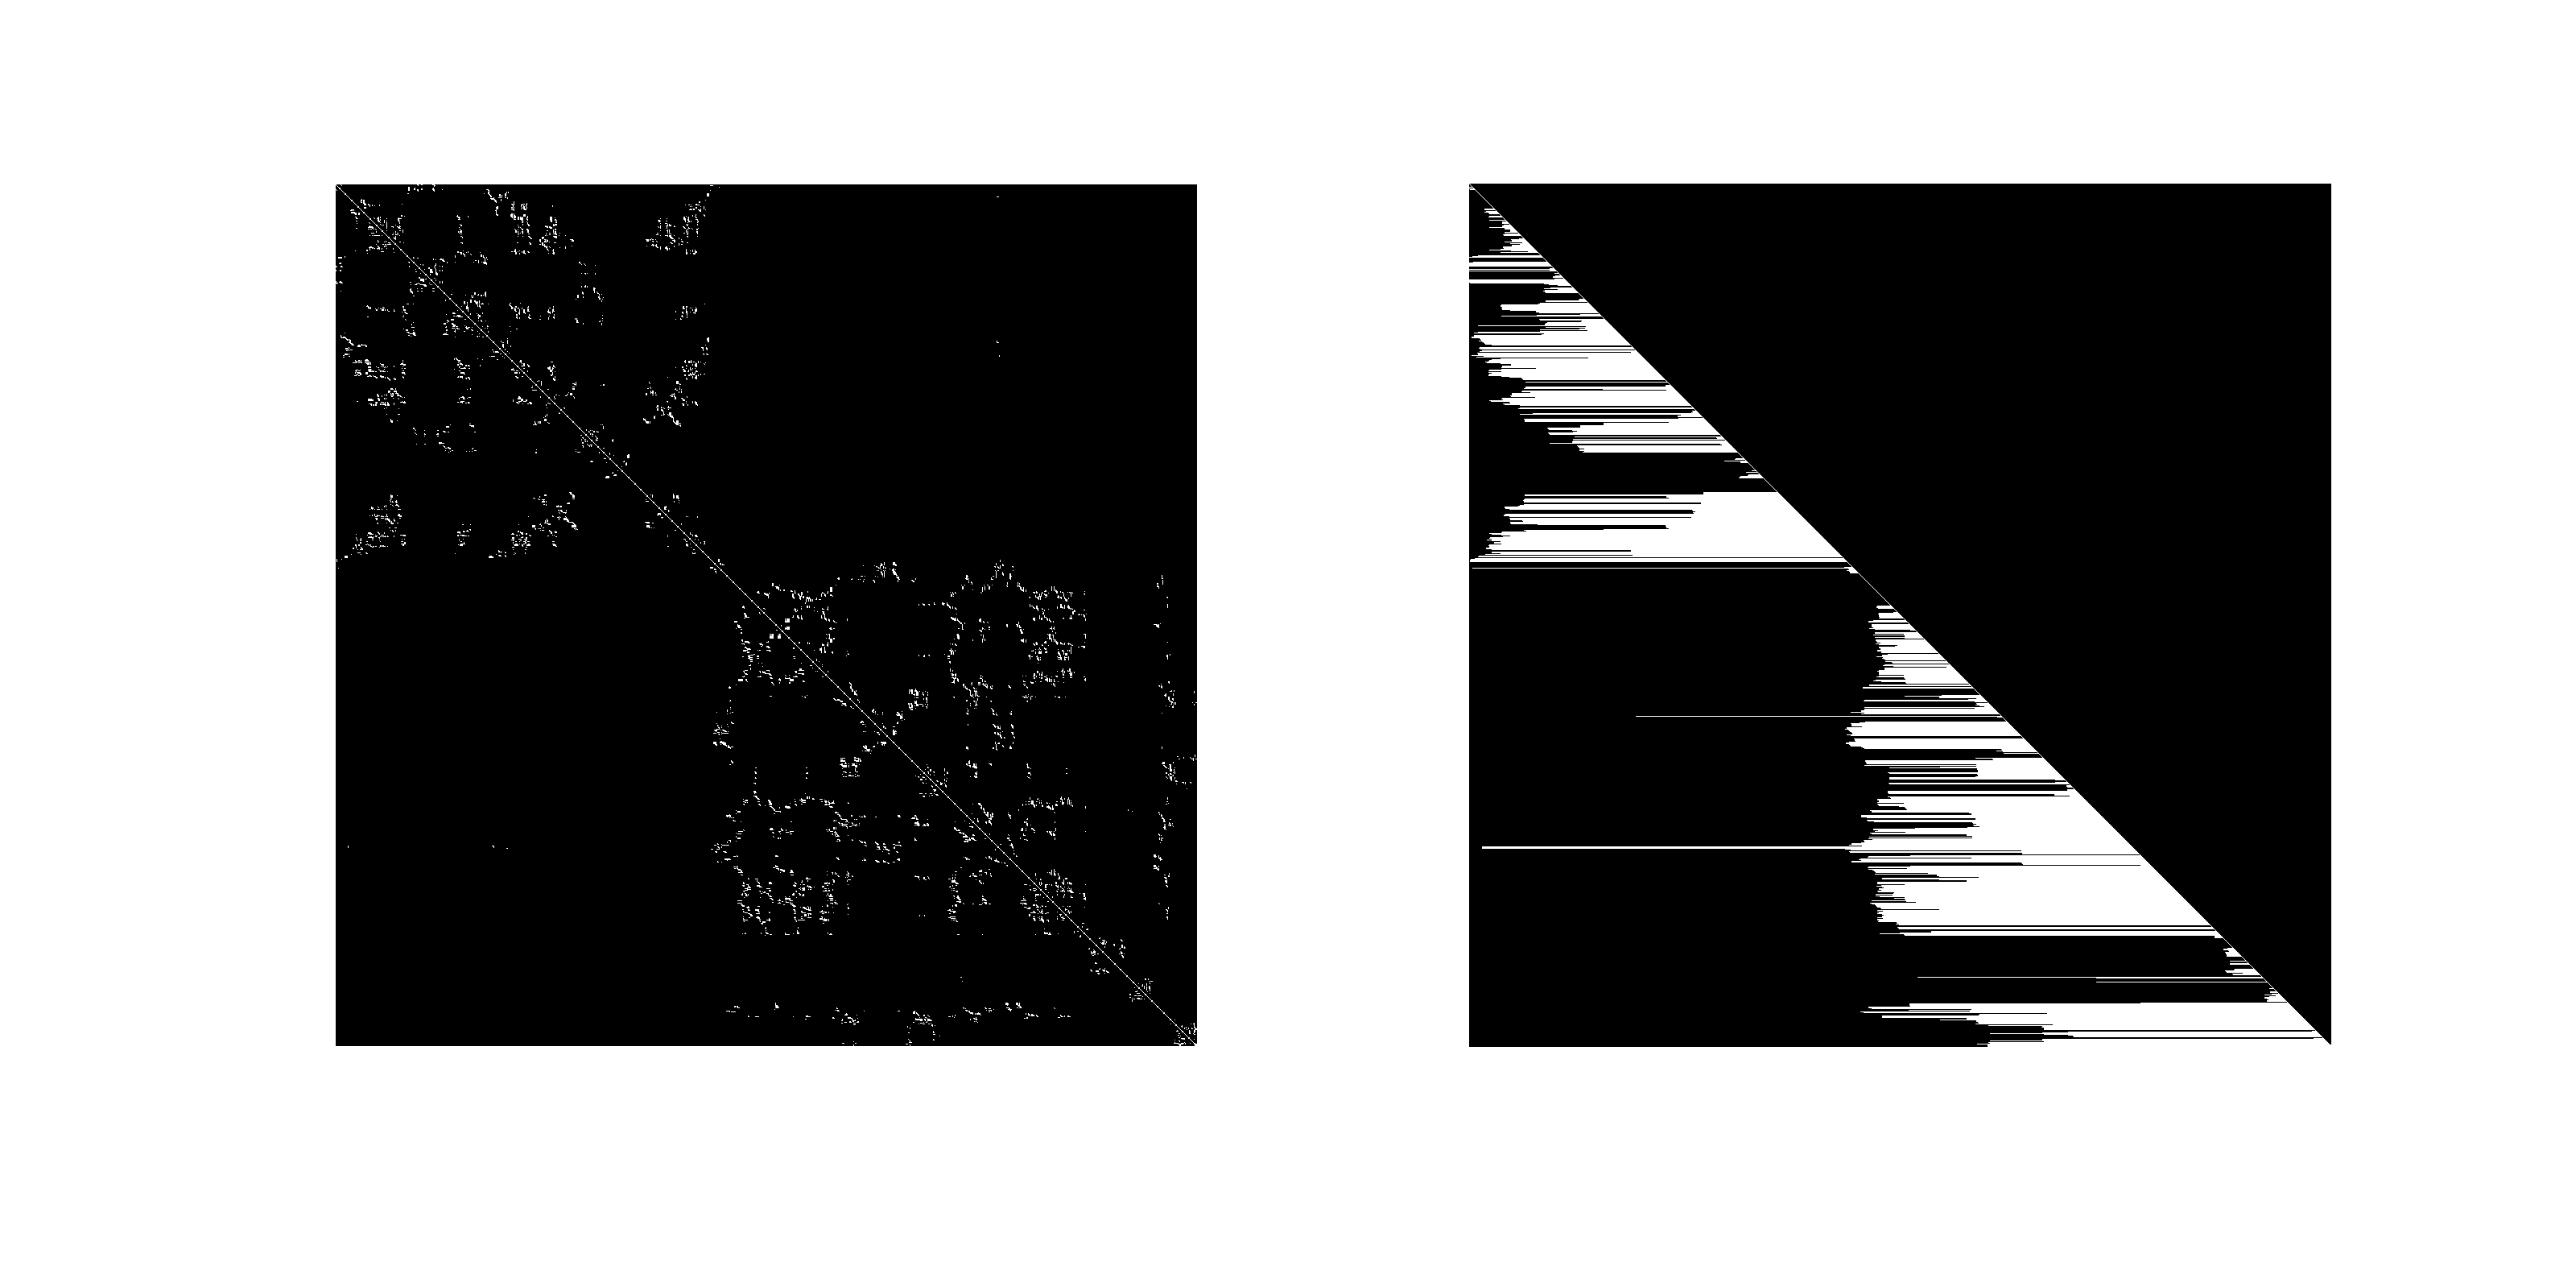
\includegraphics[width=\textwidth]{figures/04_solvingSe3/h_l_no_permutation.pdf}
        \label{fig:cholesky_fill_in_no_odering}
    \end{minipage}\\
    \begin{minipage}[t!]{\textwidth}
        \centering
        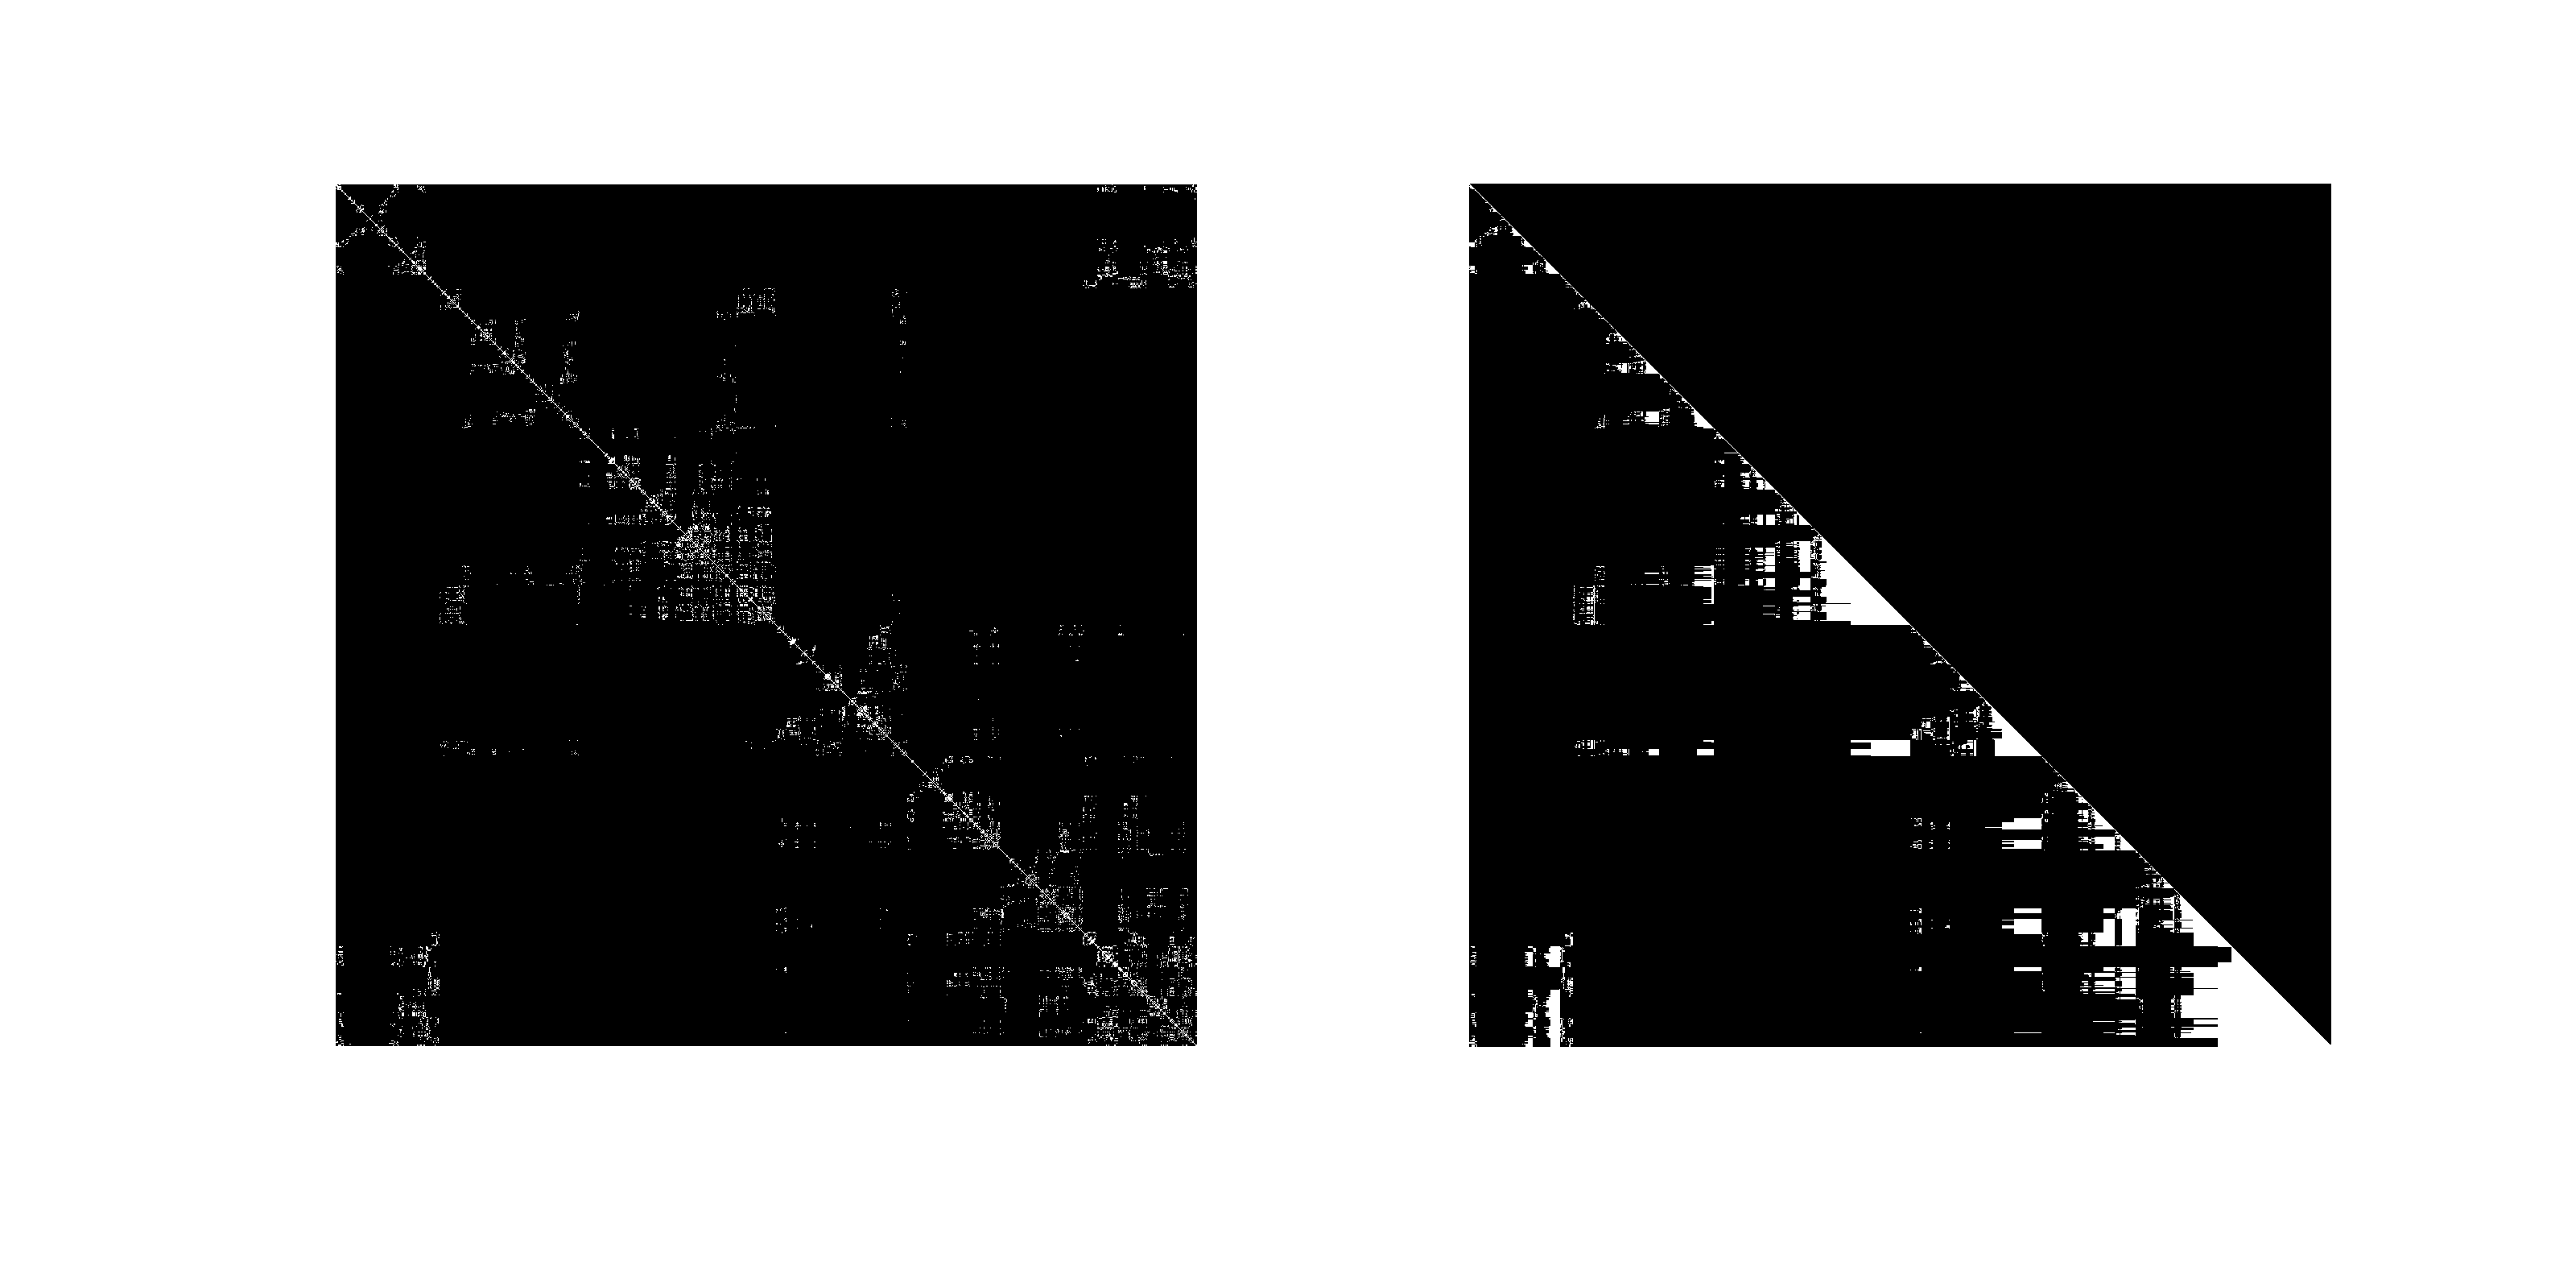
\includegraphics[width=\textwidth]{figures/04_solvingSe3/h_l_amd.pdf}
        \label{fig:cholesky_fill_in_amd}
    \end{minipage}%
    \caption{\textbf{Cholesky Fill-In.} The figure highlights the fill-in due to the factorization of a $(2000\times2000)$ symmetric PSD matrix: non-zero blocks are depicted in white, while null-blocks in black. The first row illustrates the patterns of matrices $\hessian$ and its decomposition $\L$ - respectively on the left and on the right. In the bottom row, the same matrices after the permutation of $\hessian$ using the AMD ordering. It is clear the ordering contribution in reducing the fill-in of the factorization, minimizing the memory required to store $\L$ and the number of block-matrices operations.} 
    \label{fig:cholesky_fill_in}
\end{figure}

As already mentioned in Section \ref{sec:sparse_ls}, variable reordering techniques, that consists in applying a suitable permutation to the source matrix, are able to reduce dramatically the fill-in, allowing a faster decomposition. Several algorithm are proposed in literature to compute the proper permutation - e.g. AMD, COLAMD. For the Cholesky $LU$ decomposition it is also possible to evaluate the pattern of the $L$ matrix before computing the actual decomposition, through the \textit{Symbolic Cholesky Decomposition}. The reader might appreciate the variable reordering contribution in Figure \ref{fig:cholesky_fill_in}.

In the remaining of the Section, it will be given a more detailed description on how to solve a sparse linear system using the Cholesky decomposition of the matrix $\hessian$.

\subsection{Storage Methods for Sparse Matrices}\label{subsec:sparse_storage_methods}
Another core aspect of sparse matrices is that there are several techniques to \textit{store} them more efficiently, reducing the amount of memory needed. The most general ones are \textit{Compressed Row Storage} (CRS) or \textit{Compressed Column Storage} (CCS), since they do not make any assumption on the structure of the matrix but the do not store unnecessary elements - i.e. the zeros. Those method store the matrix using only 3 vectors: one vector for floating point numbers that represent the non-zero entries and two for the column and row indexes respectively. As an example, given a matrix $A$

\begin{equation*}
    A = 
        \begin{pmatrix}
            10 & 0 & 0 & 0 & -2 & 0 \\
            3 & 9 & 0 & 0 & 0 & 3 \\
            0 & 7 & 8 & 7 & 0 & 0 \\
            3 & 0 & 8 & 7 & 5 & 0 \\
            0 & 8 & 0 & 9 & 9 & 13 \\
            0 & 4 & 0 & 0 & 2 & -1 
        \end{pmatrix}
\end{equation*}

\noindent in CRS format is represented by the following vectors - using zero-based indexing:

\begin{align*}
    val &= \begin{bmatrix}10 & -2 & 3 & 9 & 3 & 7 & \cdots & 2 & -1\end{bmatrix} \\
    col &= \begin{bmatrix}0 & 4 & 0 & 1 & 5 & 1 & \cdots & 4 & 5\end{bmatrix} \\
    row &= \begin{bmatrix}0 & 2 & 5 & 8 & 12 & 16 & 19\end{bmatrix}     
\end{align*}

\noindent The vector $row$ contains the indexes of the elements that correspond to the first non-zero entry of each row in the sparse matrix A.

\textit{List of Lists} (LIL) represents another effective and easy-to-implement storage method. In this case, each row-vector is represented as a list of pairs that denotes the column index and the element's value.

Recalling equation \ref{eq:sparse_hessian_structure}, since in this problem it has been considered only \textit{binary constraints}, the linearization of each edge generates $4$ block-contributions to the Hessian, namely:

\begin{align*}
    \hessian_{ii} &= \jacob_i^T \Omega_k \, \jacob_i \qquad
    \hessian_{jj} = \jacob_j^T \Omega_k \, \jacob_j \\
    \hessian_{ij} &= \jacob_i^T \Omega_k \, \jacob_j \qquad
    \hessian_{ji} = \jacob_j^T \Omega_k \, \jacob_i 
\end{align*}

\noindent Therefore, the Hessian can be intended to be a \textit{sparse block-matrix} where each entry is a matrix itself of a given size. In our work, it has been chosen to employ the LIL storage method with block-entries, in order to speed-up the numerical computations - better explained in the next Chapter.

\subsection{Cholesky Decomposition}\label{subsec:cholesky_dec_general}
In linear algebra, the Cholesky decomposition (or factorization) is the decomposition of a \textit{Hermitian}, positive semi-definite (PSD) matrix into the product of a \textit{lower triangular matrix} and its \textit{conjugate transpose}, namely:

\begin{empheq}[box={\mybluebox[1pt]}]{equation}
    \label{eq:generic_cholesky}
    \mathbf{A} = \L\,\L^\star
\end{empheq}

\noindent In this particular problem formulation, the matrices involved are composed by real numbers, therefore the conjugate transpose of $\L$ becomes its transposed $\L^T = \U$. In this sense, it represents the square-root operator for symmetric PSD matrices.

A more stable variant of the classical Cholesky decomposition is the \textbf{LDL} decomposition. In this case, the original matrix is decomposed into the following product:

\begin{equation}
    \label{eq:ldl_decomposition}
    \mathbf{A} = \L \mathbf{D} \L^\star
\end{equation}

\noindent where $\L$ is a lower \textit{unit} triangular matrix - i.e. all the entries on the main diagonal are $1$ - and $\mathbf{D}$ a diagonal matrix. This variant requires the same space and computational effort with respect to the original one but avoids the square-roots extraction. In this way, even matrices that do not have a Cholesky decomposition can be factorized with the \textit{LDL} one. However, in this work, since the matrices take into account are symmetric and PSD by construction, it has been chosen the original Cholesky decomposition.

In general the computational complexity for the factorization of a $(n \times n)$ matrix is $O(n^3)$, requiring about $\nicefrac{n^3}{3}$ FLOPs. There are several algorithm available to compute the factorization, however, one of the most common is the \textit{Cholesky-Banachiewicz}. In this algorithm the computation starts from the top-left corner of the matrix $\L$ and proceeds the computation row-by-row as follows:

\begin{equation*}
    \mathbf{A} = \L \L^T = 
        \begin{pmatrix}
            L_{00} & 0 & 0 \\ L_{10} & L_{11} & 0 \\ L_{20} & L_{12} & L_{22} 
        \end{pmatrix}
        \,
        \begin{pmatrix}
            L_{00} & L_{10} & L_{20} & \\ 0 & L_{11} & L_{21} \\ 0 & 0 & L_{22}
        \end{pmatrix}
\end{equation*}

\noindent where

\begin{empheq}[box={\mybluebox[3pt]}]{equation}
    \label{eq:cholesky_banachiewicz}
    \begin{cases}
        L_{jj} = \sqrt{A_{jj} - \sum_{k = 1}^{j-1}L_{j k}^2} \\
        L_{ij} = \frac{1}{L_{jj}}\left[A_{ij} - \sum_{k = 1}^{j-1}L_{ik}\,L_{jk}\right] \qquad\quad \text{for}\quad i>j
    \end{cases}
\end{empheq}

The \textit{Cholesky-Crout}'s algorithm, instead, is a column-wise version of the previous one. It is good to notice that both algorithms allow to perform the computation also \textit{in-place}. Moreover, both algorithms can be employed in sparse block-matrices, leading to a block-Cholesky factorization. The blocks are also computed as in Equation \ref{eq:cholesky_banachiewicz} but, in the block case, the \textit{square root} operator is applied to the matrix-block and it consists in the \textit{Cholesky decomposition of the block} itself.

As it has been already mentioned, the main use of the Cholesky decomposition is in the solution of linear systems. Given a symmetric PSD real matrix $\mathbf{A}$, the solution of the linear system $\mathbf{A}\,\state = \bvec$ is computed through the following steps:

\begin{enumerate}
    \item \textbf{Cholesky factorization} of the source matrix $\mathbf{A} = \L \L^T$
    \item \textbf{Forward substitution} to solve the linear system $\L \, \mathbf{y} = \bvec$
    \item \textbf{Backward substitution} to solve the linear system $\L^T\, \state = \mathbf{y}$
\end{enumerate}

Clearly, since in the problem in analysis $\hessian$ and its factorization $\L$ are sparse \textit{block-matrices}, also $\bvec$ and $\mathbf{y}$ are dense \textit{block-vector} - with the number of blocks $N$ equal to the number of vertexes in the graph.

\section{Manifold Representation}\label{sec:manifold_se3}
As it has been already stated at the begin of the Chapter, this work focuses on 3D formulations of pose-graph and bundle adjustment. In this Section it will be better analyzed the representation of all the objects required for the LS estimation in both the formulations.

\subsection{3D Pose-Graph}\label{subsec:3d_pose_graphs}
Pose-graph optimization in 3D represents the backbone of SLAM, allowing to estimate the robot trajectory \textit{in space} through MAP estimation. In this formulation, the state $\state$ includes the 3D orientation of the nodes which represent the main reason why pose-SLAM is a complex problem. Rotations in space can be over-parametrized through a 3D rotation matrix $\rot \in SO(3)$. Therefore, the over-parametrized state can be represented by a 3D isometry $\SState = \,\T{W}{R} \in SE(3)$ which represents the robot pose in the world reference frame - i.e. a $(4 \times 4)$ homogeneous transformation matrix.

A possible \textit{minimal representation} of the state can be a $6$ vector $\state = (t_x\,t_y\,t_z\,\alpha\,\beta\,\gamma)^T$, where the triplet $\mathbf{r} = (\alpha\,\beta\,\gamma)^T$ represents the Euler Angles that compose the rotational part of the isometry, while $\trans = (t_x\,t_y\,t_z)^T$ is the translational one. Summarizing, in formul\ae:

\begin{equation*}
    \SState = 
        \begin{pmatrix}
            \rot & \trans \\ \zero^T & 1
        \end{pmatrix}
    \qquad 
    \state = \begin{bmatrix} t_x & t_y & t_z & \alpha & \beta & \gamma \end{bmatrix}^T
\end{equation*}

\noindent where

\begin{equation}
    \label{eq:se3_rotation}
    \rot = \rot_x(\alpha) \, \rot_y(\beta)\, \rot_z(\gamma)
\end{equation}

The measurements are also of type \textit{pose}, thus, it is possible to use the same notation that describes the state. Therefore $\Meas_{ij}$ represents the over-parametrized measurement of node $j$ with respect to node $i$ - i.e. a 3D isometry $\T{i}{j}$.

The next required step concerns the definitions of suitable operators \textit{box-plus} and \textit{box-minus}. We introduce again the operators \textit{v2t} and \textit{t2v} that allow to map the over-parametrized representation into the minimal one and vice versa. Those two operators allow to define the following relations:

\begin{align}
    \label{eq:standard_boxplus_se3}
    \SState \boxplus \dx &= \v2t(\dx) \, \SState \\
    \label{eq:standard_boxminus_se3}
    \SState_a \boxminus \SState_b &= \text{t2v}\left(\SState_b^{-1}\SState_a\right)
\end{align}

\noindent For $SE(3)$ object, the \textit{v2t} function computes the rotational part of $\SState$ through Equation \ref{eq:se3_rotation} and then composes the isometry adding the translational part $\trans = (t_x \: t_y \: t_z)^T$. In Equation \ref{eq:se3_rotation} the factors $\rot_x$, $\rot_y$ and $\rot_z$ represent the 3D rotation respectively around the $x$, $y$ and $z$ axis; they are defined as follows:

\begin{align}
    \label{eq:rotx_3d}
    \rot_x(\alpha) &= 
        \begin{bmatrix}
            1 & 0 & 0 \\ 0 & \cos\alpha & -\sin\alpha \\ 0 & \sin\alpha & \cos\alpha
        \end{bmatrix} \\
    \label{eq:roty_3d}
    \rot_y(\beta) &=
        \begin{bmatrix}
            \cos\beta & 0 & \sin\beta \\ 0 & 1 & 0\\ -\sin\beta & 0 & \cos\beta
        \end{bmatrix} \\
    \label{eq:rotz_3d}
    \rot_z(\gamma) &= 
        \begin{bmatrix}
            \cos\gamma & -\sin\gamma & 0 \\ \sin\gamma & \cos\gamma & 0 \\ 0&0&1
        \end{bmatrix} 
\end{align}

Instead, to retrieve the Euler given the rotation matrix $\rot$ - that is done in the \textit{t2v} operator - it is necessary to equate each element in $\rot$ with its corresponding element in the matrix product $\rot_x(\alpha) \, \rot_y(\beta)\, \rot_z(\gamma)$, in formul\ae:

\begin{align}
    \label{eq:rot_composition_xyz}
    \rot &= 
        \begin{bmatrix}
            R_{00} & R_{01} & R_{02} \\
            R_{10} & R_{11} & R_{12} \\
            R_{20} & R_{21} & R_{22} 
        \end{bmatrix}
     = \rot_x(\alpha) \, \rot_y(\beta)\, \rot_z(\gamma) = \\
     &=
        \begin{bmatrix}
            \cos\beta\,\cos\gamma & -\cos\beta\,\sin\gamma & \sin\beta \\
            \cos\alpha\,\sin\gamma + \sin\alpha\,\cos\gamma\,\sin\beta & \cos\alpha\,\cos\gamma - \sin\alpha\,\sin\beta\,\sin\gamma & -\cos\beta\,\sin\alpha \\
            \sin\alpha\,\sin\gamma - \cos\alpha\,\cos\gamma\,\sin\beta & \sin\alpha\,\cos\gamma + \cos\alpha\,\sin\beta\,\sin\gamma & \cos\beta\,\cos\alpha 
        \end{bmatrix} \nonumber
\end{align}

The reader might notice the non-linearities introduced by the functions t2v and v2t. Those imply the computation of complex non-linear derivatives to retrieve the Jacobian in the linearization phase. However, this problem - and the solution proposed in this work - will be better analyzed in the next Section.

\subsection{3D Bundle Adjustment}\label{subsec:3d_bundle_adj}
In this formulation, as already explained in Section \ref{sec:bundle_adjustment_problem}, the system has to estimate both the robot trajectory and the position of salient world points - i.e. the 3D landmarks. Therefore, the system's \textit{state} and \textit{increment} are described as follows:

\begin{align*}
    \SState &= \left(\overbracket{\SState^R_1, ..., \SState^R_N}^{N poses}\: |\: \overbracket{\state^L_{N+1}, ..., \state^L_{N+M}}^{M landmarks}\right) \\
    \dx &= \left(\overbracket{\dx^R_1, ..., \dx^R_N}^{N poses}\: |\: \overbracket{\dx^L_{N+1}, ..., \dx^L_{N+M}}^{M landmarks}\right)
\end{align*}

The formalization for $SE(3)$ nodes remains unchanged from the previous Sub-Section, therefore, it is necessary to characterize only the nodes that describe the landmarks. 

Landmarks' nodes lie on $\mathbb{R}^3$, so it is not necessary to define anything else - i.e. no \textit{box-plus}/\textit{box-minus} operator needed. As a consequence of this, a measurement $\meas_{ij} \in \mathbb{R}^3$ is a simple 3 vector that describes the position of point $j$ in the $i$-th pose reference frame.

However, it is necessary to consider also the fact that the sensor's reference frame and the robot's one might not coincide, but they are related through the transformation $\S = \,\T{R}{S} \in SE(3)$. Thus, given the state, the \textit{predicted measurement} is:

\begin{equation}
    \label{eq:prediction_se3r3}
    \tmeas_{ij} = h_{ij}(\SState) = \underbracket{\S^{-1}\,\SState_i^{-1}}_{\mathbf{K}}\p_j = \rot_{K}\p_j + \trans_K
\end{equation}

\noindent In light of this, without loss of generality, the error between the predicted and the actual measurement is computed as follows:

\begin{empheq}[box={\mybluebox[0pt]}]{equation}
    \label{eq:error_se3r3}
    \error_{ij} = \tmeas_{ij} - \meas_{ij} = \S^{-1}\SState_i^{-1}\p_j - \meas_{ij}
\end{empheq}

\noindent Given Equation \ref{eq:error_se3r3}, the perturbed error will be:

\begin{equation}
    \label{eq:perturbed_error_se3r3}
    \error_{ij}(\SState_i \boxplus \dx_i^R, \state_j + \dx_j^L) = \S^{-1}\left[\left(\v2t(\dx_i^R)\SState_i\right)^{-1}\left(\p_j+\dx_j^L\right)\right] - \meas_{ij}
\end{equation}

Finally, it is necessary to compute the Jacobian $\jacob$ deriving from the constraint $\meas_{ij}$, that is structured as follows:

\begin{equation*}
    \jacob = \left[\zero \: \cdots \: \zero \:\, \jacob_R \,\: \zero \: \cdots \: \zero \:\, \jacob_L \,\: \zero \: \cdots \: \zero\right]
\end{equation*}

\noindent where

\begin{align*}
    \jacob_R &= \frac{\partial\,\S^{-1} \left[\left(\v2t(\dx_i^R)\SState_i\right)^{-1}\left(\p_j + \dx_j^L\right) - \meas_j\right]}{\partial\dx_i^R} \Bigg \rvert_{\scriptsize\begin{matrix} \dx_i^R = 0\\\dx_j^L = 0\end{matrix}} = \\
    &= \frac{\partial\: \left[\rot_{S}^T\left[\v2t(\dx_i^R) \SState_i\right]^{-1} \, \p_j - \rot_{S}^T\trans_S\right]}{\partial\dx_i^R} \Bigg \rvert_{\scriptsize\begin{matrix} \dx_i^R = 0\\\dx_j^L = 0\end{matrix}} = \\
    &= \frac{\partial\, \rot_{S}^T \SState_i^{-1} \left[\v2t(\dx_i^R)\right]^{-1} \, \p_j}{\partial\dx_i^R} \Bigg \rvert_{\scriptsize\begin{matrix} \dx_i^R = 0\\\dx_j^L = 0\end{matrix}} = \\
    &= \frac{\partial\, \left[\rot_{S}^T\, \rot_{R}^T\, \left[\v2t(\dx_i^R)\right]^{-1} \, \p_j - \rot_{R}^T\,\trans_R\right]}{\partial\dx_i^R}\Bigg \rvert_{\scriptsize\begin{matrix} \dx_i^R = 0\\\dx_j^L = 0\end{matrix}} = \\
    &= \frac{\partial\, \rot_{S}^T \, \rot_{R}^T \left(\left[\v2t(\dx_i^R)\right]^{-1} \, \p_j\right)}{\partial\dx_i^R} \Bigg \rvert_{\tiny\begin{matrix} \dx_i^R = 0\\\dx_j^L = 0\end{matrix}} =
    \rot_{S}^T \, \rot_{R}^T \frac{\partial\, \left[\rot_{\dx_i^R} \,\p_j - \rot_{\dx_i^R} \,\trans_{\dx_i^R}\right]}{\partial\dx_i^R} \Bigg \rvert_{\tiny\begin{matrix} \dx_i^R = 0\\\dx_j^L = 0\end{matrix}} 
\end{align*}

\noindent Exploiting the fact that the derivative expressed in the previous equation is evaluated in $\dx_i^R = 0$, it leads to the following relation:

\begin{empheq}[box={\mybluebox[0pt]}]{equation}
    \label{eq:jac_r_se3r3}
    \jacob_R = \rot_{S}^T \: \rot_{R}^T \: \begin{bmatrix} -I_{3\times3} & | & -{\lfloor\p_j\rfloor}_\times\,\end{bmatrix}
\end{empheq}

\noindent The other component of $\jacob$ - namely $\jacob_L$ - instead can be computed as follows:

\begin{align*}
    \jacob_L &= \frac{\partial\,\S^{-1} \left[\left(\v2t(\dx_i^R)\SState_i\right)^{-1}\left(\p_j + \dx_j^L\right) - \meas_j\right]}{\partial\dx_j^L} \Bigg \rvert_{\scriptsize\begin{matrix} \dx_i^R = 0\\\dx_j^L = 0\end{matrix}} = \\
    &= \frac{\partial\,\left[\rot_{S}^T \, \SState_i^{-1}\left(\p_j + \dx_j^L\right) - \rot_{S}^T \, \trans_S\right]}{\partial\dx_j^L} \Bigg \rvert_{\scriptsize\begin{matrix} \dx_i^R = 0\\\dx_j^L = 0\end{matrix}} = \\
    &= \frac{\partial\,\left[\left(\rot_{S}^T \, \SState_i^{-1}\p_j\right) +  \left(\rot_{S}^T \, \SState_i^{-1}\dx_j^L\right)\right]}{\partial\dx_j^L} \Bigg \rvert_{\scriptsize\begin{matrix} \dx_i^R = 0\\\dx_j^L = 0\end{matrix}} = 
    \rot_{S}^T \, \frac{\partial\,\left[\rot_R^T \, \dx_j^L  - \rot_{R}^T\trans_R\right]}{\partial\dx_j^L} \Bigg \rvert_{\scriptsize\begin{matrix} \dx_i^R = 0\\\dx_j^L = 0\end{matrix}} 
\end{align*}

%\dx_i^R = 0, \dx_j^L = 0

\noindent This result - expanding the derivatives and exploiting that the linearization point is $\dx_j^L = 0$ - leads to the following relation:

\begin{empheq}[box={\mybluebox[0pt]}]{equation}
    \label{eq:jac_l_se3r3}
    \jacob_L = \rot_{S}^T\:\rot_{R}^T
\end{empheq}

\noindent The reader might notice that $\jacob_R$ is a $(3 \times 6)$ matrix - since the minimal representation of $SE(3)$ states has $6$ components - while $\jacob_L$ is a $(3\times3)$ matrix - because $\mathbb{R}^3$ states are vectors with only $3$ components. 

\vspace{15px}

In the next Section it is proposed a deeper analysis on the error representation and the linearization of 3D pose constraints, highlighting the non-linearity of the computation and the proposed approach to overcome this issue.

\section{Dealing with SE3 Objects}{\label{sec:se3_objects}}
3D poses are complex objects to manage, due to their rotational part that introduces many an highly non-linear contribution in the linearization process. In this section it is proposed an approach that aims to reduce those non-linearities while delivering performances comparable to other state-of-the-art systems.

\subsection{Chordal Distance Based Error Function}\label{subsec:chordal_dist_error}
Recalling \ref{subsec:3d_pose_graphs}, we have defined the functions v2t and t2v that allow to map the minimal representation of the state into the redundant one and vice-versa. Through them, we defined the operators \textit{box-plus} and \textit{box-minus}, described respectively in Equations \ref{eq:standard_boxplus_se3} and \ref{eq:standard_boxminus_se3}. Sticking to this notion, the \textit{predicted measurement} $\Pred_{ij}$ of pose $j$ from pose $i$ is computed as

\begin{equation}
    \label{eq:standard_prediction_se3}
    \Pred_{ij} = h_{ij}(\SState) = \SState_i^{-1}\SState_j
\end{equation}

\noindent that leads to the following error function:

\begin{equation}
    \label{eq:standard_error_se3}
    \error_{ij}(\SState) = \Pred_{ij} \boxminus \Meas_{ij} = \text{t2v}\left(\Meas_{ij}^{-1}\: \SState_i^{-1} \: \SState_j\right)
\end{equation}

\noindent The error $\error_{ij}$ is a 6 vector that expresses the mismatch of each component of state's minimal representation. Proceeding with the error perturbation, the result will be:

\begin{equation}
    \label{eq:standard_perturbated_error_se3}
    \error_{ij}(\SState_i \boxplus \dx_i, \SState_j \boxplus \dx_j) = \text{t2v}\left(\Meas_{ij}^{-1}\left(\v2t(\dx_i)\,\SState_i\right)^{-1} \, \left(\v2t(\dx_j)\,\SState_j\right)\right)
\end{equation}

The full Jacobian $\jacob = \left[\zero \: \cdots \: \zero \:\, \jacob_i \,\: \zero \: \cdots \: \zero \:\, \jacob_j \,\: \zero \: \cdots \: \zero\right]$  will be quite complex to compute due to the derivative of the t2v and v2t functions, requiring also many FLOPs and, thus, slowing the optimization process. In this formulation $\jacob_i$ and $\jacob_j$ are $(6\times6)$ matrices.

It is possible to approach this problem using a different error formulation that leads to easy-to-compute derivatives. In order to do so, we define the $L_{p,q}$ norm of a $(m\times n)$ matrix $A$ as follows:

\begin{equation*}
    \norm{A}_{p,q} = \left(\sum_{j=1}^{n} \left(\sum_{i=1}^{m} |a_{ij}|^p \right)^{\nicefrac{q}{p}}\right)^{\nicefrac{1}{q}}
\end{equation*}

\noindent For $p = q = 2$ the becomes

\begin{empheq}[box={\mybluebox[2pt]}]{equation}
    \label{eq:frobenius_norm}
    \norm{A}_F = \left( \sum_{j=1}^{n} \left(\sum_{i=1}^{m}|a_{ij}|^2 \right)^{\nicefrac{2}{2}}\right)^{\nicefrac{1}{2}} = \sqrt{\sum_{i=1}^{m}\:\sum_{j=1}^{n}|a_{ij}|^2}
\end{empheq}

\noindent that represents the \textit{Frobenius norm} of a matrix, an \textit{entrywise} norm, which is also \textit{invariant under rotation} constraint. Based on this concept, it is possible to define the \textit{chordal distance} between two rotation matrix $\rot_{A}$ and $\rot_{B}$ as follows:

\begin{equation}
    \label{eq:chordal_distance_true}
    d_{\text{chord}}(\rot_{A}, \rot_{B}) = \norm{\rot_{A} - \rot_{B}}_F
\end{equation}

\noindent It is good to notice that the difference operator employed in Equation \ref{eq:chordal_distance_true} is the standard Euclidean \textit{minus}, executed element-wise.

\begin{figure}[!hbt]
    \centering
    \resizebox{0.7\textwidth}{!}{\input{figures/04_solvingSe3/chordal_distance.pdf_tex}}
    \caption{\textbf{Chordal Distance.} This figure shows the underlying concept of the new error function: the distance between $\mathbf{p}_1$ and $\mathbf{p}_2$ can be approximated with the Euclidean distance computed between the projection of those points onto the relative chord - namely between $\hat{\mathbf{p}}_1$ and $\hat{\mathbf{p}}_2$.} 
    \label{fig:chordal_distance}
\end{figure}

We define also a new function, that given a 3D isometry returns a 12 vector made with its components, namely:

\begin{align}
    \SState &= 
        \begin{bmatrix}
            \rot & \trans \\ \zero & 1
        \end{bmatrix} \nonumber \\
    \rot &= \begin{pmatrix} \mathbf{r}_1 | \mathbf{r}_2 | \mathbf{r}_3 \end{pmatrix} \nonumber \\
    \text{flatten}(\SState) &= \begin{pmatrix} \mathbf{r}_1 \\ \mathbf{r}_2 \\ \mathbf{r}_3 \\ \trans \end{pmatrix}
    \label{eq:flatten_isometry_operator}
\end{align}

\noindent where $\mathbf{r}_k$ represents the $k$-th column of $\rot$.

Finally, we introduce the following relations to express operators \textit{box-plus} and \textit{box-minus}:

\begin{align}
    \label{eq:boxplus_se3}
    \SState \boxplus \dx &= \v2t(\dx)\, \SState \\
    \label{eq:boximus_se3}
    \SState_a \boxminus \SState_b &= \flatten{\SState_a} - \flatten{\SState_b}
\end{align}

Given those mathematical concepts, it is possible to define the error between two $SE(3)$ objects through a relaxed version of the chordal distance, that leads to the following relations:

\begin{align}
    \label{eq:prediction_se3}
    \Pred_{ij} = h_{ij}(\SState) &= \flatten{\SState_i^{-1}\,\SState_j} \\
    \label{eq:error_se3}
    \error_{ij}(\SState) = \Pred_{ij} - \Meas_{ij} &= \flatten{\SState_i^{-1}\, \SState_j} - \flatten{\Meas_{ij}}
\end{align}

\noindent It is good to notice that $\error_{ij}$ now is a 12 vector, therefore, the Jacobian's components $\jacob_i$ and $\jacob_j$ will be $(12\times6)$ matrices. Speaking about this, applying the state perturbation to the error will lead to the following relation:

\begin{equation}
    \label{eq:perturbed_error_se3}
    \error_{ij}(\SState_i \boxplus \dx_i, \SState_j \boxplus \dx_j) = \flatten{\left(\v2t(\dx_i)\SState_i\right)^{-1}\,\left(\v2t(\dx_j)\SState_j\right)} - \flatten{\Meas_{ij}}
\end{equation}

\noindent It is already possible to notice the reduced complexity of the derivatives required to linearize the constraint. In fact, from Equation \ref{eq:perturbed_error_se3} it is possible to retrieve the following relations - stating that $\rot_{\dx_i} = \rot_{\dx_i}^x \, \rot_{\dx_i}^y \, \rot_{\dx_i}^z$:

\begin{align*}
    \jacob_j &= \frac{\partial\: \error_{ij}(\SState_i \boxplus \dx_i, \SState_j \boxplus \dx_j)}{\partial \dx_j} \Bigg \rvert_{\scriptsize\begin{matrix} \dx_i = 0\\\dx_j = 0\end{matrix}} = \\
    &= \frac{\partial \left[\flatten{\overbracket{\begin{bmatrix}\rot_i^T & -\rot_i^T \trans_i \\\zero & 1\end{bmatrix} \begin{bmatrix}\left(\rot_{\dx_i}^x \, \rot_{\dx_i}^y \, \rot_{\dx_i}^z\right)^T & -\rot_{\dx_i}^T \trans_i \\\zero & 1\end{bmatrix} \begin{bmatrix}\rot_j & \trans_j \\\zero & 1\end{bmatrix}}^{\mathbf{G}}}\right]}{\partial \dx_j} \Bigg \rvert_{\scriptsize\begin{matrix} \dx_i = 0\\\dx_j = 0\end{matrix}} 
\end{align*}

\noindent Expanding the derivatives, it is possible to define the following - intuitively retrieved - objects:

\begin{itemize}
    \item  $\rot_{x0}^{\prime}$, $\rot_{y0}^{\prime}$ and $\rot_{z0}^{\prime}$ that represent derivatives with respect to $\Delta\alpha$, $\Delta\beta$ and $\Delta\gamma$ of the base rotation $\rot_k(\cdot)$, evaluated in 0 and with $k = \{x,y,z\}$;
    \item  $\hat{\rot}_{x0}^{\prime}$, $\hat{\rot}_{y0}^{\prime}$, and $\hat{\rot}_{z0}^{\prime}$ that are the derivatives with respect to $\Delta\alpha$, $\Delta\beta$ and $\Delta\gamma$ of the rotational part of matrix $\mathbf{G}$, computed as $\hat{\rot}_{k0}^{\prime} = \rot_{i}^T \, \rot_{k0}^{\prime} \, \rot_j$ with $k = \{x,y,z\}$;
    \item $\hat{\mathbf{r}}_{k0}^{\prime}$ which describes the 9 vector obtained stacking the columns of $\hat{\rot}_{k0}^{\prime}$ - with $k = \{x,y,z\}$.
\end{itemize}

\noindent In the light of what we just stated, it is possible to retrieve this final formulation of $\jacob_j$:

\begin{empheq}[box={\mybluebox[3pt]}]{equation}
    \label{eq:jac_j_se3} 
    \jacob_j = 
        \begin{pmatrix}
            \zero_{(9\times3)} & \begin{bmatrix} \hat{\mathbf{r}}_{x0}^{\prime} & | & \hat{\mathbf{r}}_{y0}^{\prime} & | & \hat{\mathbf{r}}_{z0}^{\prime} \end{bmatrix}_{(9\times3)} \\
            \rot_{i}^T & -\rot_{i}^T \, \skew{\trans_j}
        \end{pmatrix}
\end{empheq}

\noindent Intuitively, the other component of the Jacobian will be simply

\begin{empheq}[box={\mybluebox[3pt]}]{equation}
    \label{eq:jac_i_se3}
    \jacob_i = -\jacob_j
\end{empheq} 

The reader might noticed how the new error function reduced the computational cost of the derivatives, due to the elimination of the highly non-linear function t2v. Moreover, the use of standard Euclidean \textit{minus} operator to express differences between transforms, leads to a better approximation by the first-order Taylor expansion of the perturbed error. This better approximation enlarges the converge basin of the optimization process and it improves the avoidance of local minima.

\subsection{Benefits in the Re-linearization}\label{subsec:benefits}
The reader might remember that, since also the measurements live on a non-Euclidean space, it is necessary to project the measurement information matrices through the \textit{box-minus} operator. Therefore, using the standard \textit{box-minus} described in Equation \ref{eq:standard_boxminus_se3} and given $\Pred_{ij}$ associated to $\Meas_{ij} = \Meas_{k}$, it is required to compute the following objects \textbf{at each iteration} of the LS optimization:

\begin{align}
    \label{eq:jacobian_meas_se3}
    \jacob_{\Meas_{k}} &= \frac{\partial \left(\Pred_{ij} \boxminus \Meas\right)}{\partial \Meas} \bigg\rvert_{\Meas = \Meas_{k}} \\
    \label{eq:std_adapted_information_matrix_se3}
    \tilde{\Omega}_k &= \left(\jacob_{\Meas_{k}} \: \Omega_k \: \jacob_{\Meas_{k}}^T\right)^{-1}
\end{align}

The error function based on the chordal distance that has been proposed in the previous Sub-section, brings benefits also in this sense. In fact, since the operator employed to compute the error is the standard Euclidean \textit{minus}, it is not required to recompute the information matrix $\Omega_k$ at each iteration. 

It is good to notice that the information matrix associated with the measurement $\Meas_{k}$ is a $(6\times6)$ matrix $\Omega_k$ , since the state's minimal representation has dimension $6$ in this formalization. However, it is necessary to consider the contribute of function $\flatten{\cdot}$ in this process: the new error space has dimension $12$, thus it is necessary to project the information matrix into the new higher dimensional space. To this end, it will be proposed now some new mathematical concepts useful in order to estimate the result of applying a non-linear transformation to a probability distribution function. 

Given a Gaussian distribution $p(x) = \mathcal{N}(x; \mu, \Sigma)$ with mean $\mu$ and covariance $\Sigma$, it is possible to represent it through a set of weighted points called \textit{Sigma Points}. Each Sigma Point $\chi^i$ is described by a set of parameters:

\begin{itemize}
    \item a \textbf{position} $x^i$
    \item a \textbf{weight for the mean} $w_m^i \in \mathbb{R}^+$
    \item a \textbf{weight for the covariance} $w_c^i \in \mathbb{R}^+$
\end{itemize}

\noindent Clearly, the conversion from the original parameters $(\mu, \Sigma)$ to the Sigma Points $\chi^i = (x^i, w_m^i, w_c^i)$ must be invertible. In fact, it is possible to reconstruct the Gaussian parameters from the Sigma Points as follows:

\begin{align}
    \label{eq:sigma_to_mean}
    \mu &= \sum_i w_m^i \: x^i \\ 
    \label{eq:sigma_to_covariance}
    \Sigma &= \sum_i w_c^i\:(x^i - \mu)(x^i - \mu)^T
\end{align}

It is good to notice that, if the original Gaussian distribution has dimension $n$, a suitable number of Sigma Point required to approximate it without loosing information will be $N = 2n + 1$. In order to control how far the Sigma Points are sampled from the mean $\mu$ though, it is possible to tune the scalar parameters $\kappa \in \mathbb{R}^+$ and $\alpha \in (0,1]$. Therefore, the position of each Sigma Point is computed as follows:
\begin{align}
    \label{eq:sigma_point_pos_0}
    x^{(0)} &= \mu \\
    \label{eq:sigma_point_pos_i}
    x^{(i)} &= 
    \begin{cases}
        \mu + [L]_i \qquad \quad \text{for} \: i \in [1 \dots n] \\
        \mu - [L]_{n-i} \qquad \text{for} \: i \in [n+1 \dots 2n]
    \end{cases}
\end{align}

\noindent where $L = \sqrt{(n + \lambda)\Sigma}$ and $\lambda = \alpha^2 (n + \kappa) - n$. Given the scalar parameter $\beta = 2$ - tuned for Gaussian PDFs - the weights are retrieved as follows:

\begin{align}
    \label{eq:sigma_point_wm_0}
    w_m^{(0)} &= \frac{\lambda}{\lambda + n} \\
    \label{eq:sigma_point_wc_0}
    w_c^{(0)} &= w_m^{(0)} + (1 - \alpha^2 + \beta) \\
    \label{eq:sigma_point_weights_i}
    w_c^{(i)} = w_m^{(i)} &= \frac{1}{2(n + \lambda)}
\end{align}

This transformation between actual Gaussian parameters and the Sigma Points is called \textbf{Unscented Transform} \cite{julier2002scaledUT}. The core feature of this mathematical function is that it can be used to apply a transformation to a PDF in a straightforward way. Sticking to Gaussian PDFs, given $X_a \sim \mathcal{N}(x_a; \mu_a, \Sigma_a)$ and its Unscented Transform $x_a \sim \mathcal{UT}(x_a; x_a^{(i)}, w_m^{(i)}, w_c^{(i)})$, computing the Gaussian $X_b = g(X_a)$ can require a lot of effort. However, a good approximation of $X_b$ can be computed applying the function $g(\cdot)$ to the Unscented Transformation of $X_a$. This translates in the application of the $g(\cdot)$ function to each Sigma Point of $x_a$, namely

\begin{empheq}[box={\mybluebox[3pt]}]{equation}
    \label{eq:pdf_function_UT}
    \chi_b^{(i)} = g\left(\chi_a^{(i)}\right) \qquad i = 1 \dots N
\end{empheq}

Going back to our problem, it is possible to transform the information matrix of each measurement $\Omega_k$ through the Unscented Transform. The required steps are the following:

\begin{enumerate}
    \item Compute the $N = 2n+1$ Sigma Points $\chi_{original}^{(i)} = (x_{original}^{(i)}, w_m^{(i)}, w_c^{(i)})$ from $\mathcal{N}(\mu_k, \Sigma_k)$, where $n$ is the minimal representation's dimension (in this case $n = 6$), $\mu_k = \text{t2v}(\Meas_{k})$ and $\Sigma_k = \Omega_k^{-1}$.
    \item Compute the new position of $\chi_{transformed}^{(i)}$ as $x_{transformed}^{(i)} = \flatten{\v2t(x_{original}^{(i)})}$.
    \item Reconstruct the new Gaussian $\mathcal{N}(\bar{\mu}_k, \bar{\Sigma}_k)$ from the Sigma Points $\chi_{transformed}^{(i)}$, leaving the parameters $w_m^{(i)}$ and $w_c^{(i)}$ unchanged.
\end{enumerate}

The adapted information matrix $\bar{\Omega}_k = \bar{\Sigma}_k^{-1}$ is a $(12\times12)$ matrix. However, since we are mapping a 6-dimensional space in a 12-dimensional space with only $N = 2n + 1 = 13$ Sigma Points, it is possible to retrieve covariance matrix subject to (multiple) rank-loss. Therefore, it is necessary to add a non-zero scalar $\epsilon$ to the main diagonal of $\bar{\Sigma}_k$, in order to avoid numerical issues during its inversion.

\begin{figure}[!hbt]
    \centering
    \begin{minipage}[t!]{0.9\textwidth}
        \centering
        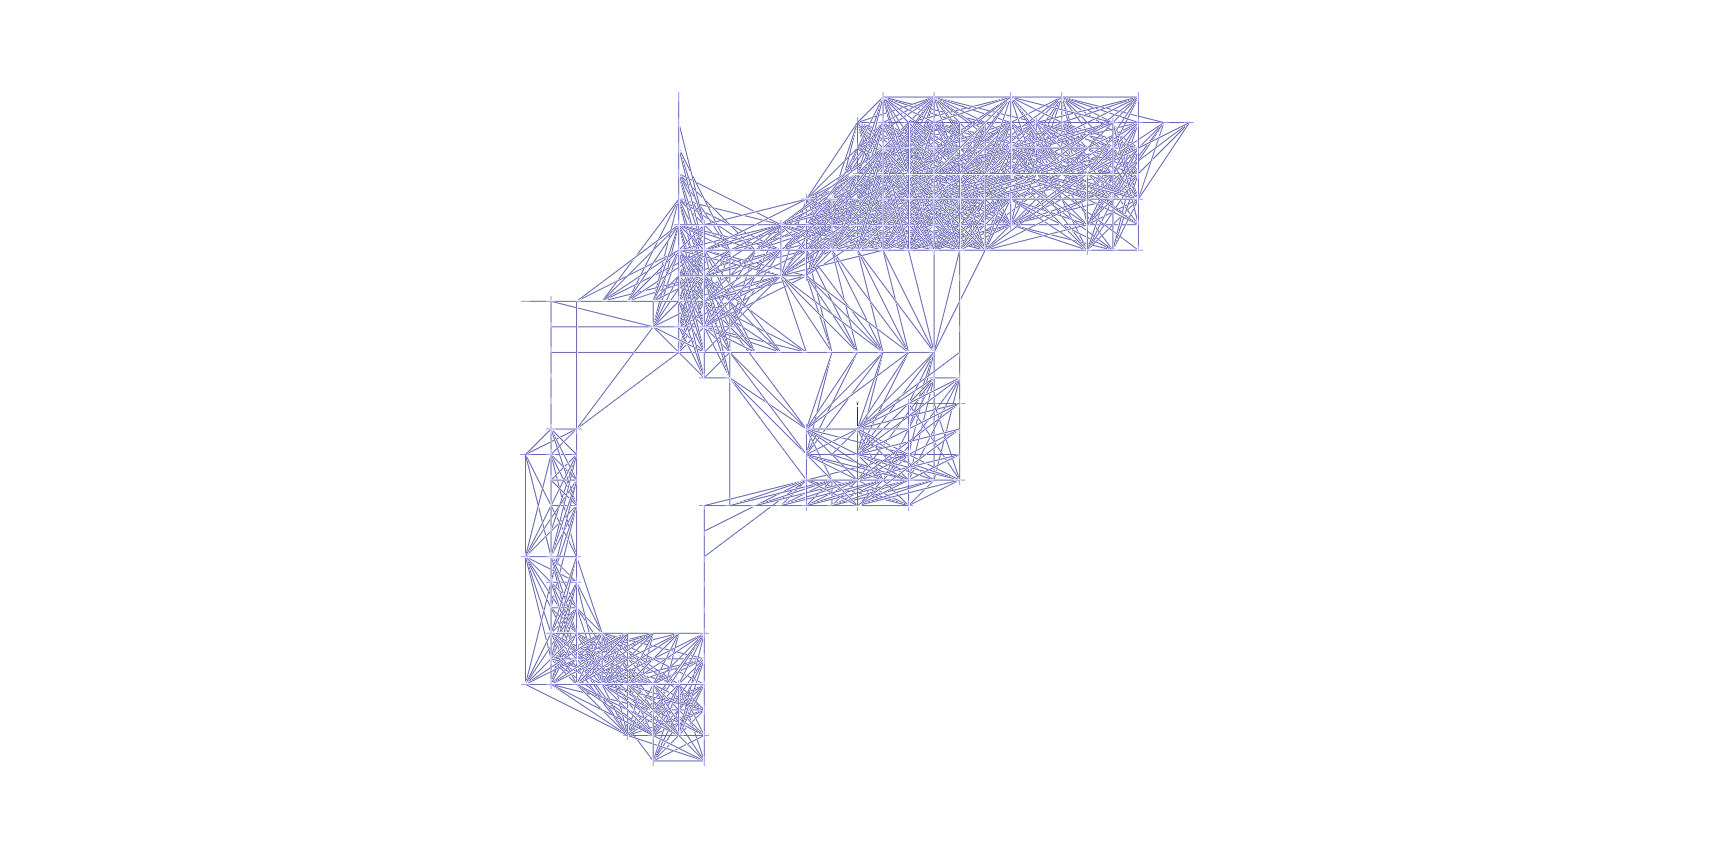
\includegraphics[width=\textwidth]{figures/04_solvingSe3/viewer_500p.png}
        \subcaption{}
        \label{fig:500p_solved}
    \end{minipage}\\
    \begin{minipage}[t!]{0.9\textwidth}
        \centering
        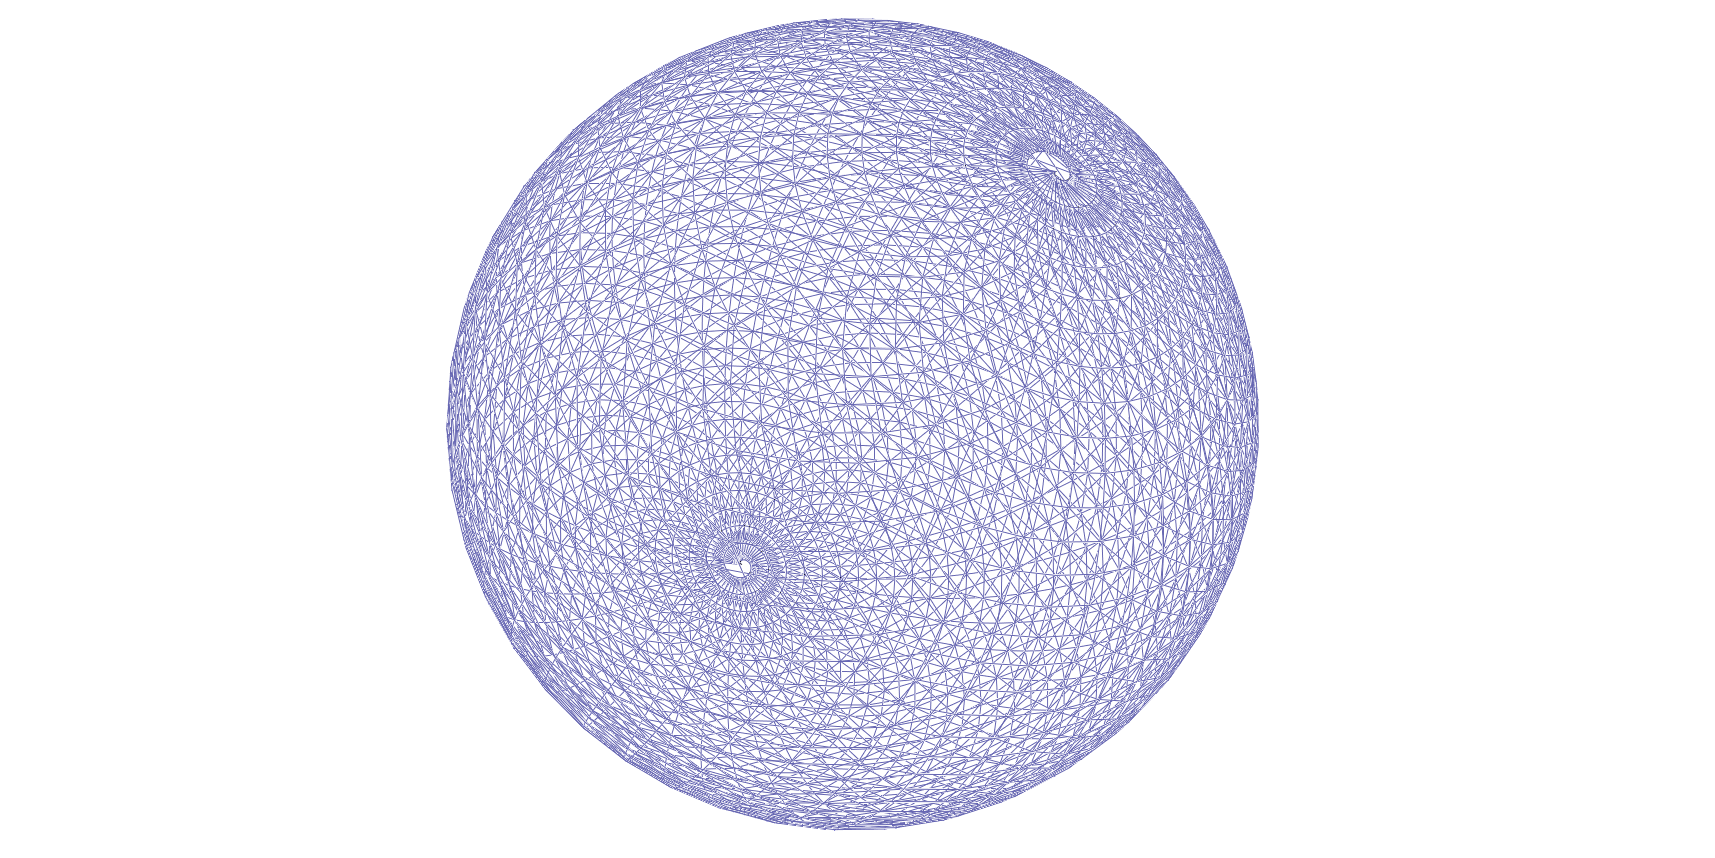
\includegraphics[width=\textwidth]{figures/04_solvingSe3/viewer_sphere.png}
        \subcaption{}
        \label{fig:sphere_solved}
    \end{minipage}%
    
    \caption{\textbf{Solved Graphs} Top image: the synthetic world graph solved. Bottom: synthetic sphere solved.} 
    \label{fig:solved_graphs}
\end{figure}

Thanks to the Unscented Transform it is possible to have a fast and quite accurate approximation of the adapted information matrix, leading to consistent results from the optimization process. Moreover, since the minus operator employed in this formulation is the standard Euclidean one, the computation is performed just one time for each measurement $\Meas_{k}$, reducing the computational effort of each optimization step.

\section{Convergence Results}\label{sec:convergence_results}
In the previous Sections, it has been proposed to the reader a complete overview of the theory underlying our optimization system. This Section, instead, proposes some tangible results brought by the novel approach described in this work.

To test the convergence of the system, we took two reference pose-graphs and we add to them different kind of noises in order to create multiple initial guess for the optimization algorithm. The graphs used are:

\begin{enumerate}
    \item \textbf{Synthetic world:} that has 501 vertices and 4277 measurements (easier);
    \item \textbf{Synthetic sphere:} 2500 vertexes and 9799 edges (hard).
\end{enumerate}

\noindent Figure \ref{fig:solved_graphs} shows the two graphs solved.
Here we propose the comparison between our system and the state-of-the-art optimizer \texttt{g2o} \cite{kummerle2011g}.

The first test done consisted in applying the noise only on the \textit{translational part} of the nodes; the employed graph is the synthetic world - Figure \ref{fig:500p_solved}. Obviously, both the system preformed well recreating the original graph, as shown in Figure \ref{fig:500p_st_solution}.

\begin{figure}[!hbt]
    \centering
    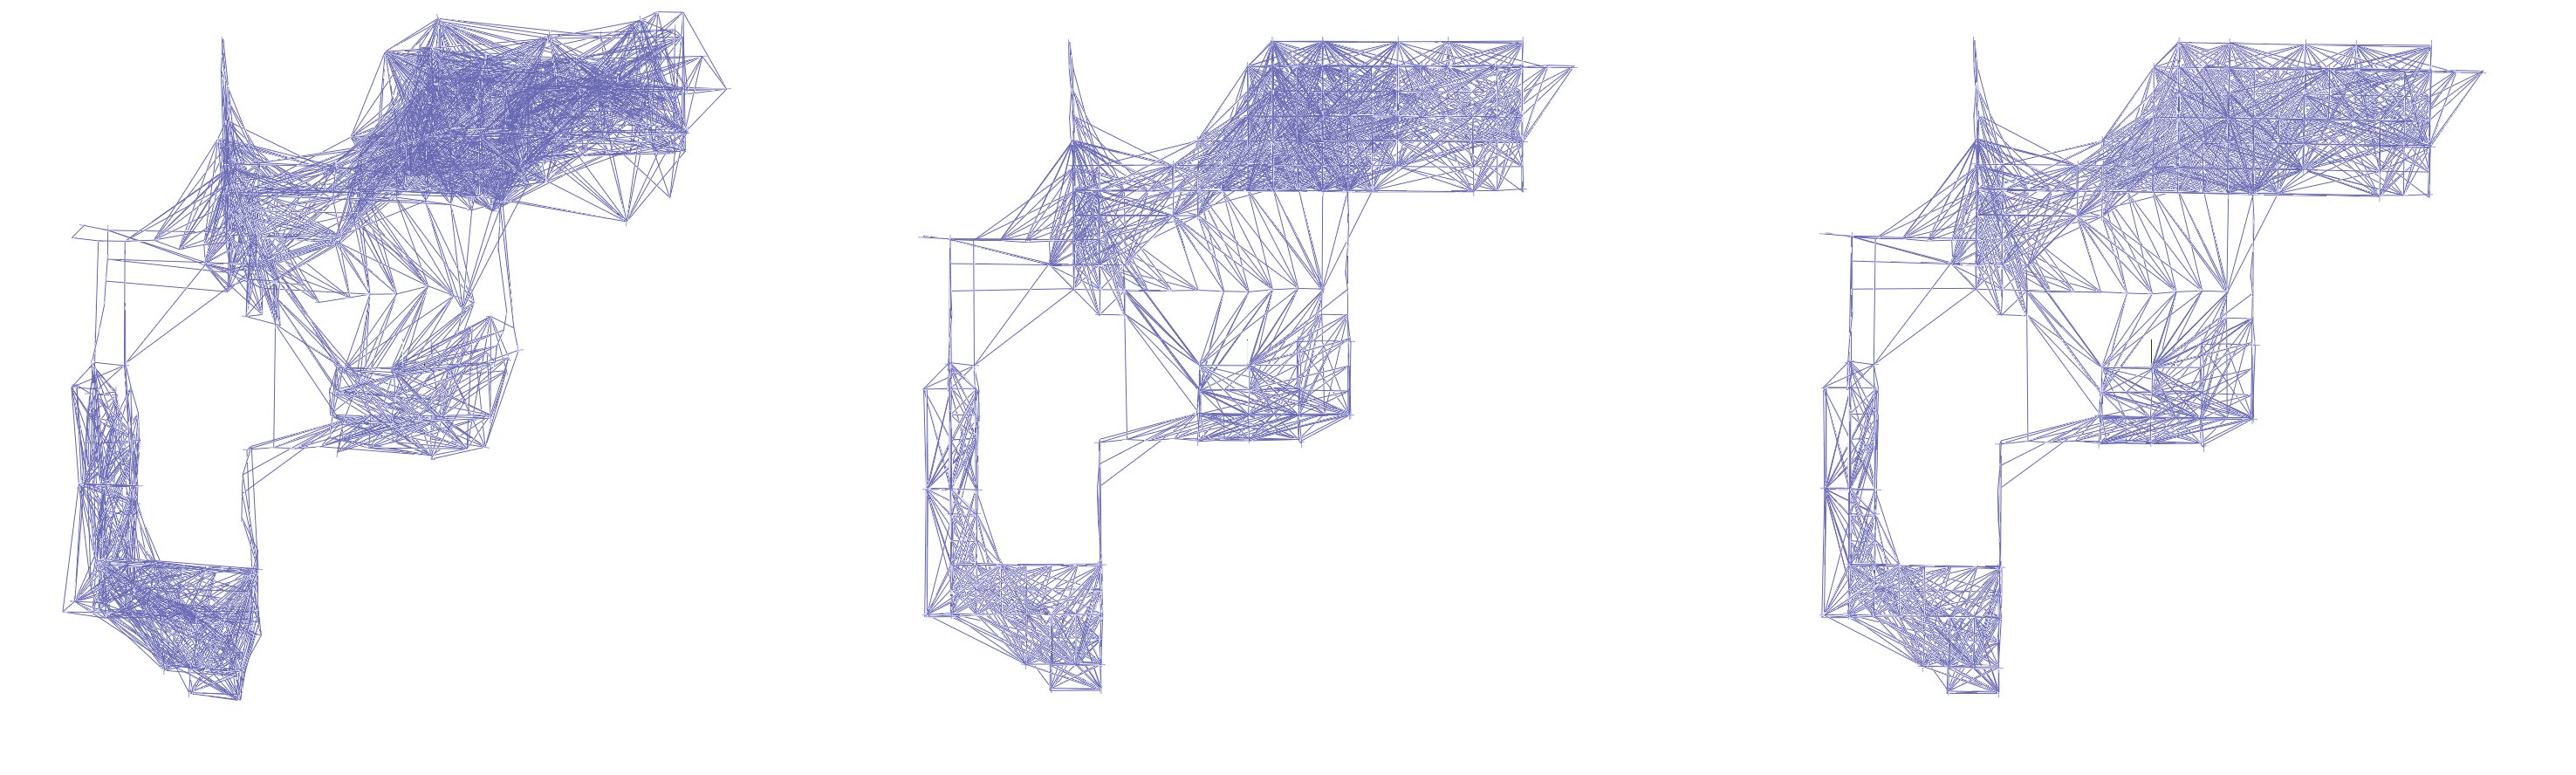
\includegraphics[width=\textwidth]{figures/04_solvingSe3/viewer_500p_st_SOLVED.png}
    \caption{\textbf{Translational Noise.} From left to right: \textit{initial guess}, \texttt{g2o} solution, \textit{our} solution. Both the approaches generate consistent results.} 
    \label{fig:500p_st_solution}
\end{figure}

However, our system claims to be more effective to manipulate rotations. Consequently, the second test focused on this: the initial guess, in fact, was created from the \textit{synthetic world} graph adding white noise - i.e. sampled from $\mathcal{N}(0,1)$ - \textit{only} to the rotation $\rot$ of each node.

\begin{figure}[!hbt]
    \centering    
    \begin{minipage}[t!]{0.9\textwidth}
        \centering
        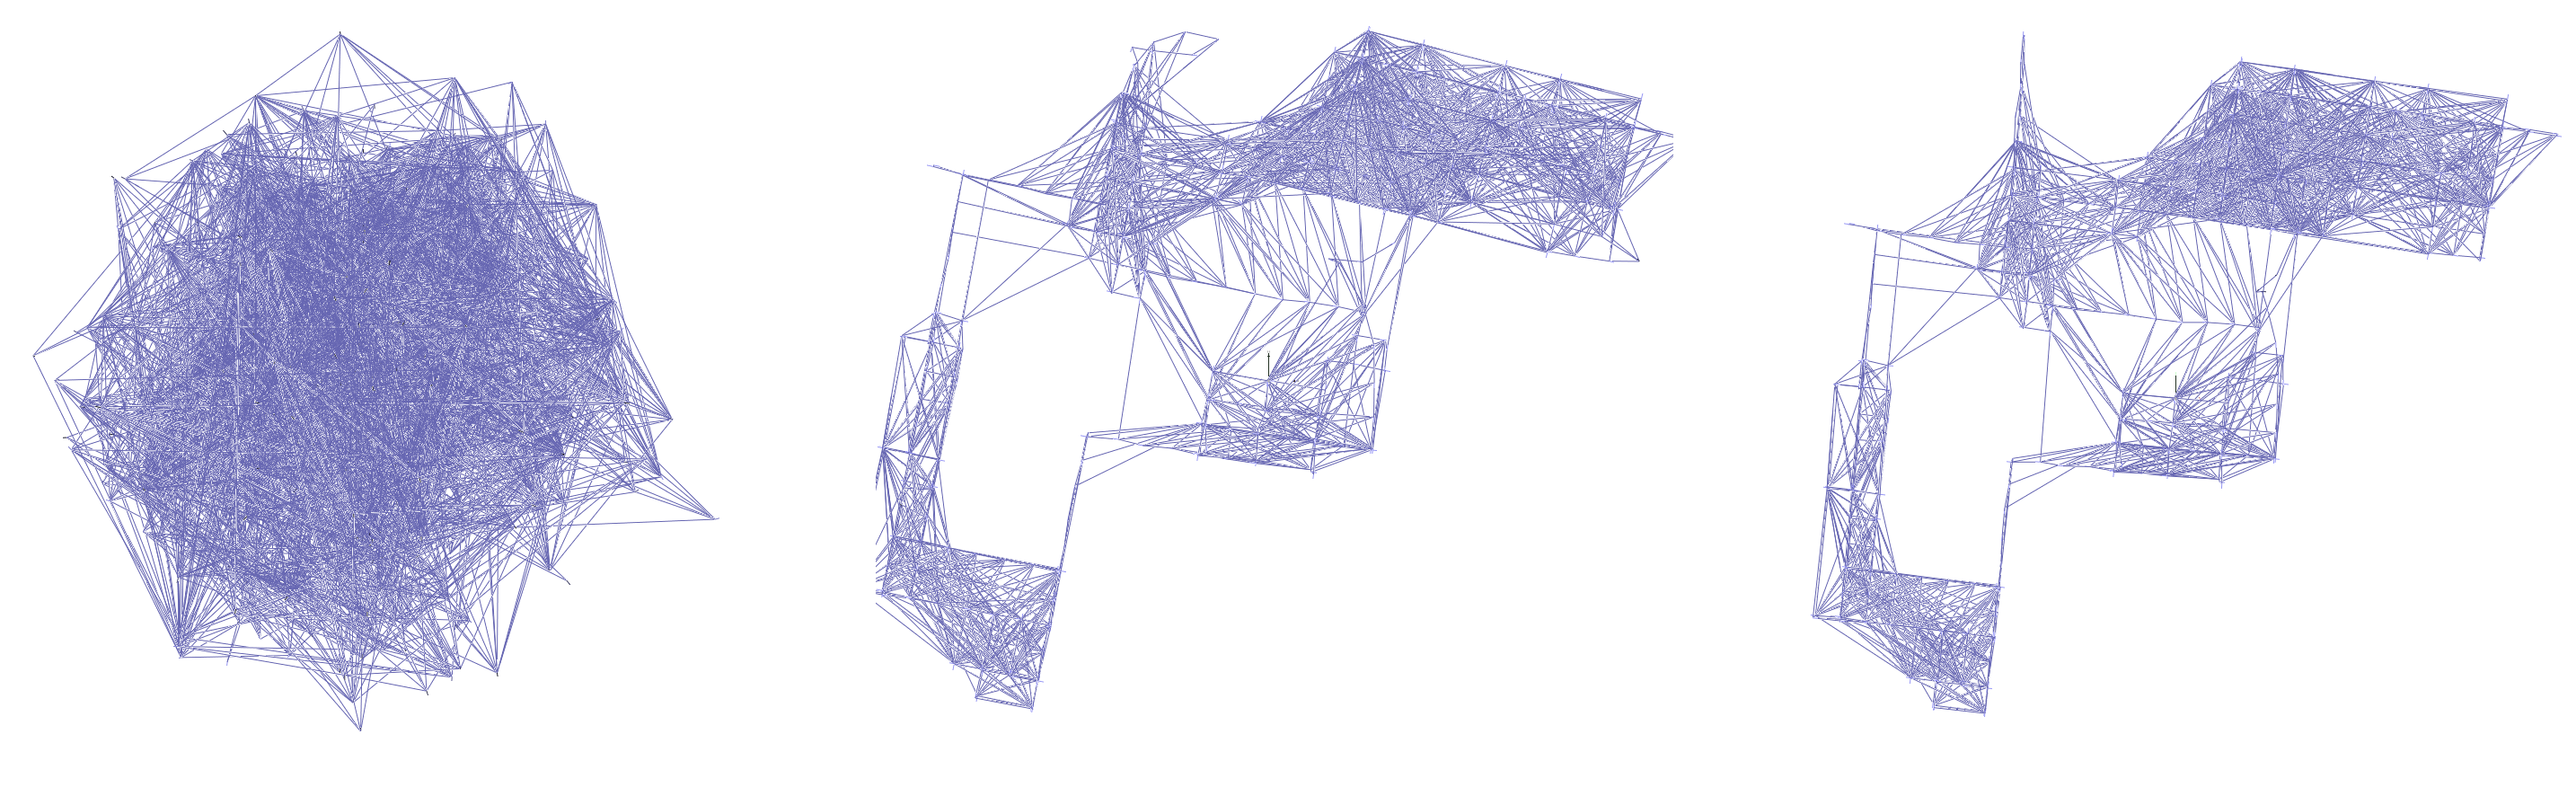
\includegraphics[width=\textwidth]{figures/04_solvingSe3/viewer_500p_awgn_SOLVED.png}
        \subcaption{} 
        \label{fig:500p_awgn_solution}
    \end{minipage}\\
    \begin{minipage}[t!]{0.9\textwidth}
        \centering
        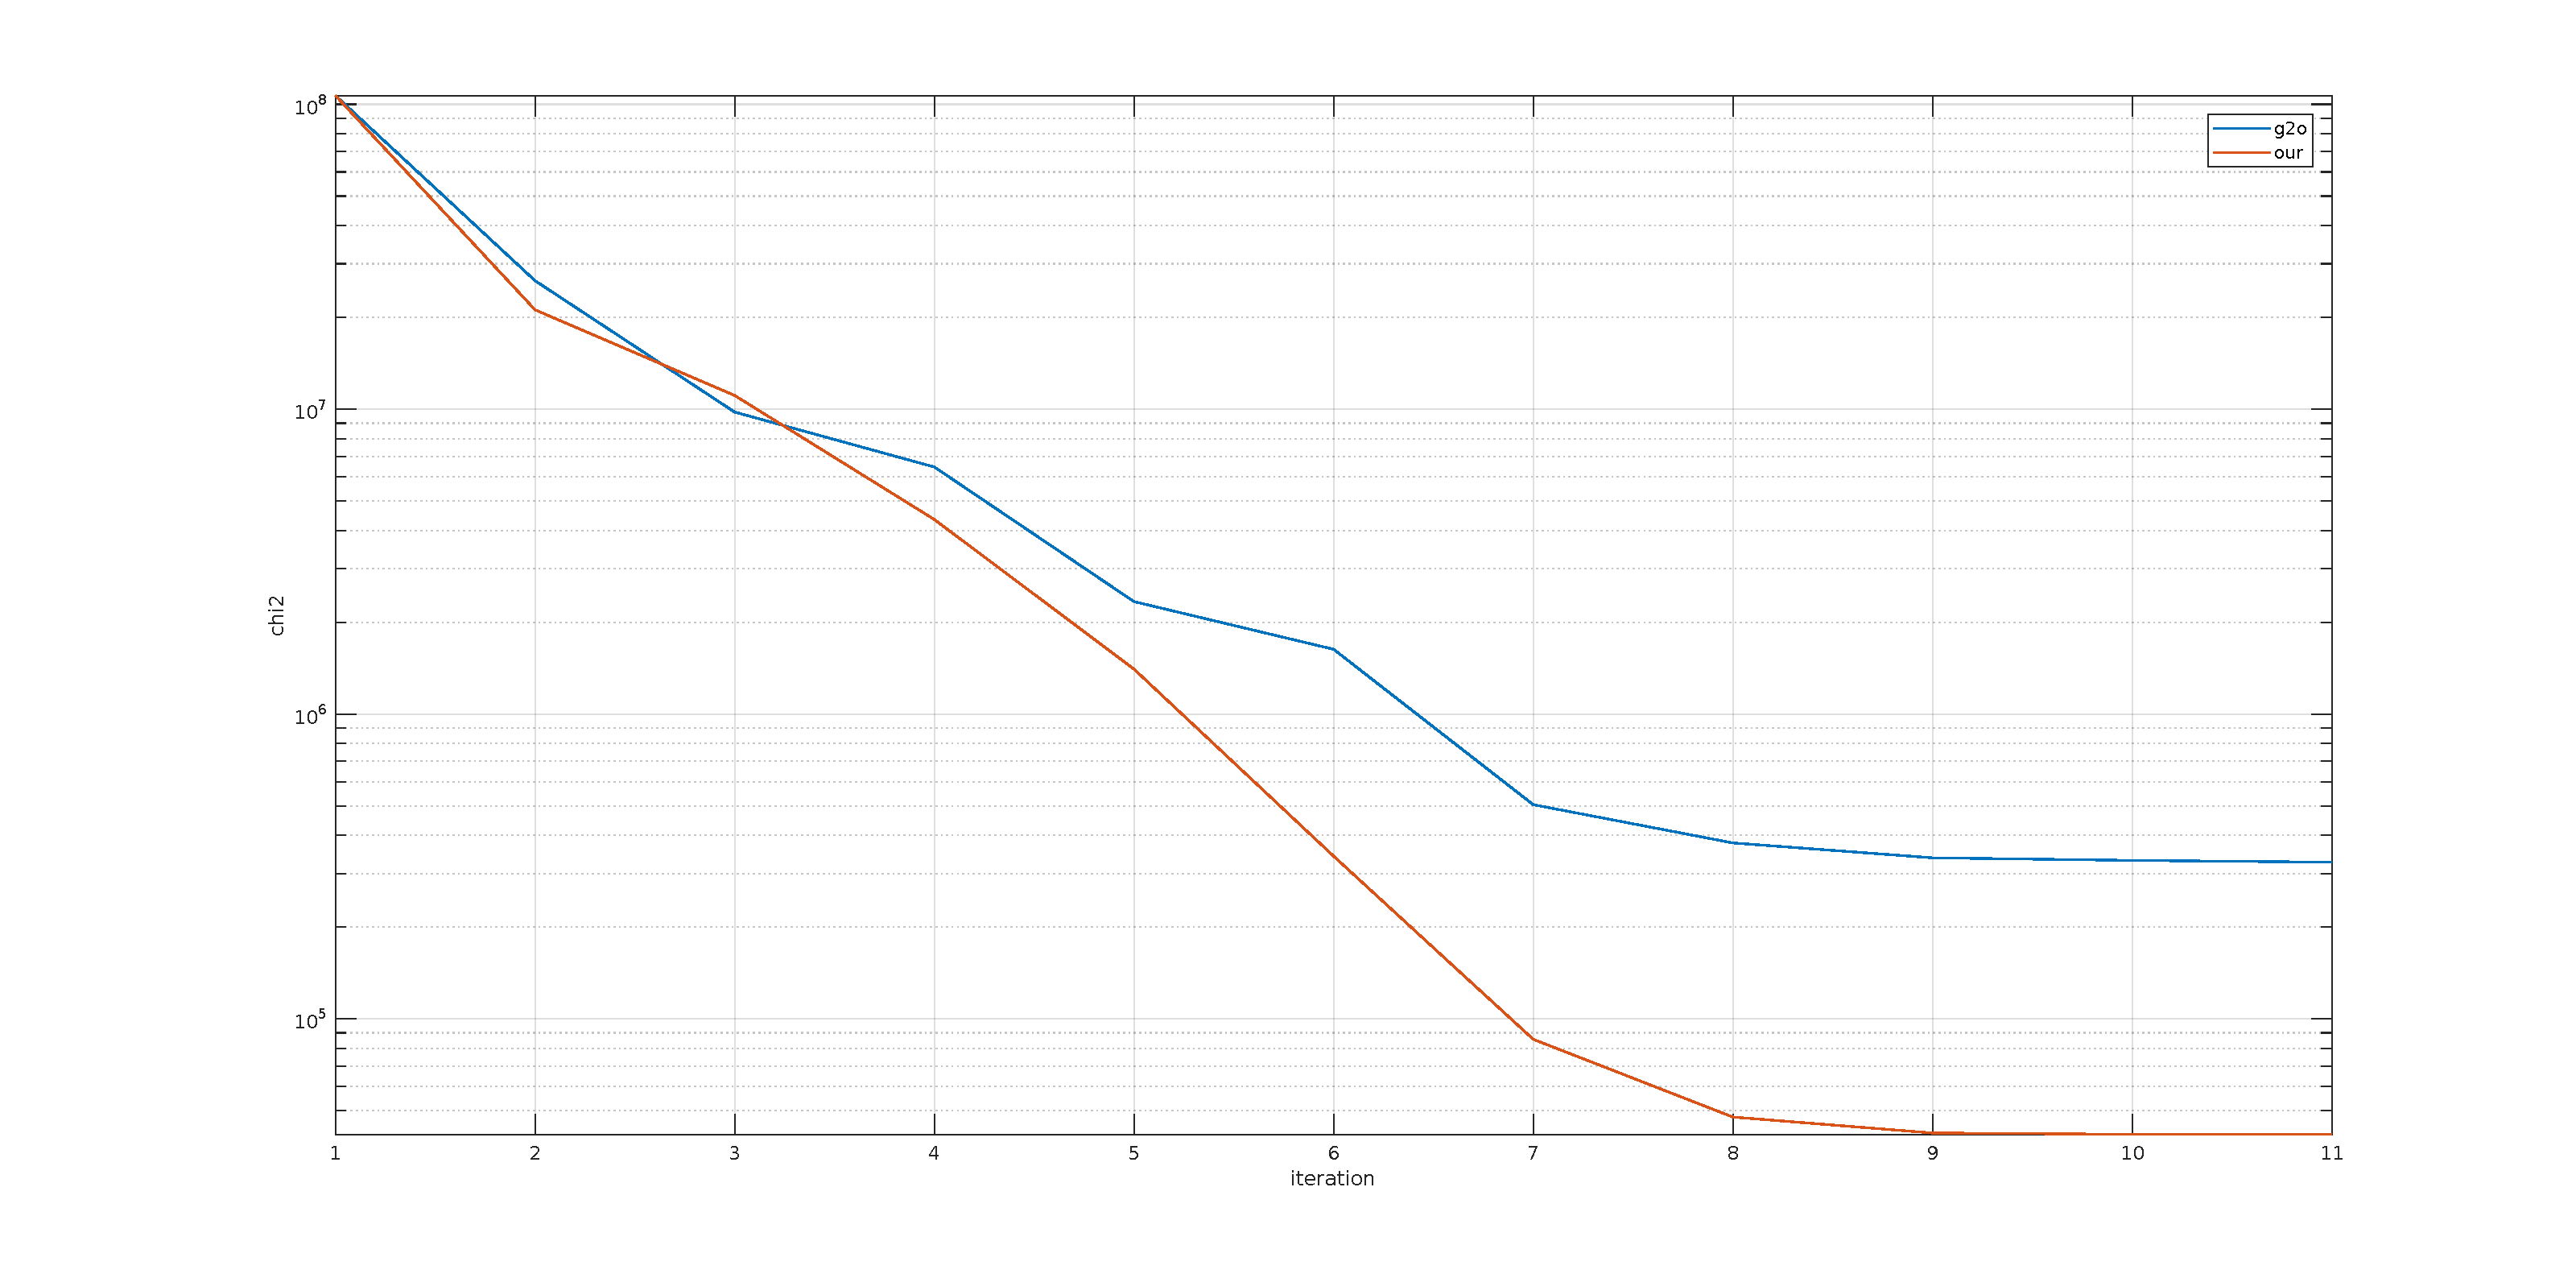
\includegraphics[width=\textwidth]{figures/04_solvingSe3/500p_N0_1.pdf}
        \subcaption{}
        \label{fig:500p_awgn_chi2}
    \end{minipage}%
    \caption{\textbf{Rotational Noise.} Figure (A) from left to right: \textit{initial guess}, \texttt{g2o} solution, \textit{our} solution. Figure (B) shows the \texttt{chi2} of both approaches at each iteration: it is clear the convergence gap between \g2o - in blue - and our approach - in orange. The $y$ axis' scale is logarithmic. The iterations performed are 10, therefore, the point $x = 1$ indicates the \texttt{chi2} of the initial guess.}
    \label{fig:500p_awgn}
\end{figure}

With this initial guess, \g2o suffers from the non-linearities introduced by the $\v2t$ and $\text{t2v}$ functions as the reader might notice in Figure \ref{fig:500p_awgn_solution}. To confirm the qualitative result obtained, we decided to compare \g2o's \texttt{chi2} with the one obtained with our approach, iteration by iteration. In order to obtain comparable objects - and to not bias the comparison - it has been saved the graph obtained with our system at each iteration and evaluated its \textit{initial} \texttt{chi2} in \g2o. The result of this comparison is shown in figure \ref{fig:500p_awgn_chi2}.

In order to further confirm the quality of the chosen approach, is has been generated another initial guess for the same graph, but the noise figure was sampled from $\mathcal{N}(0, 1000)$. In this case both the systems struggle to find a solution in only 10 iterations, but the trend is better with our error function - see Figure \ref{fig:500p_gnadvanced}.

\begin{figure}[!hbt]
    \centering    
    \begin{minipage}[t!]{0.45\textwidth}
        \centering
        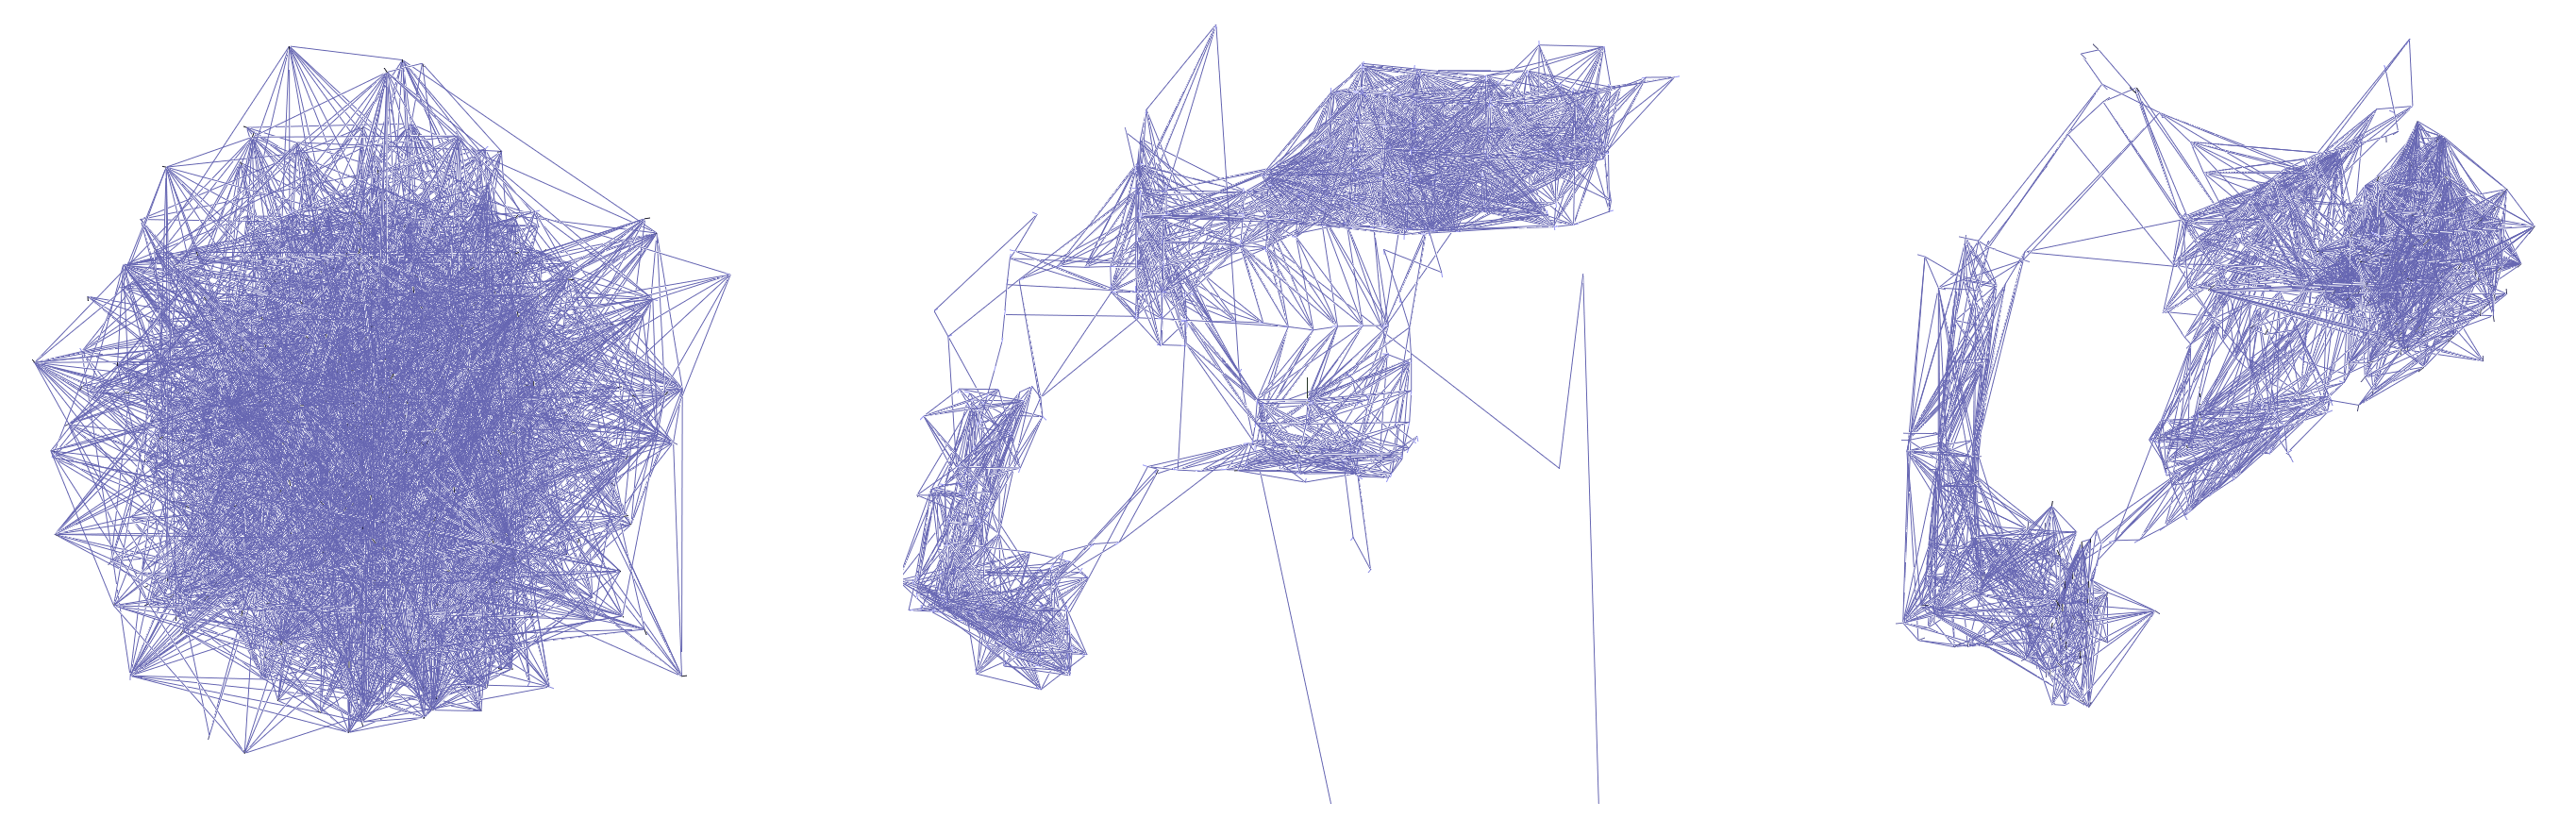
\includegraphics[width=\textwidth]{figures/04_solvingSe3/viewer_500p_gnadvanced_SOLVED.png}
        \subcaption{} 
        \label{fig:500p_gnadvanced_solution}
    \end{minipage}
    \begin{minipage}[t!]{0.45\textwidth}
        \centering
        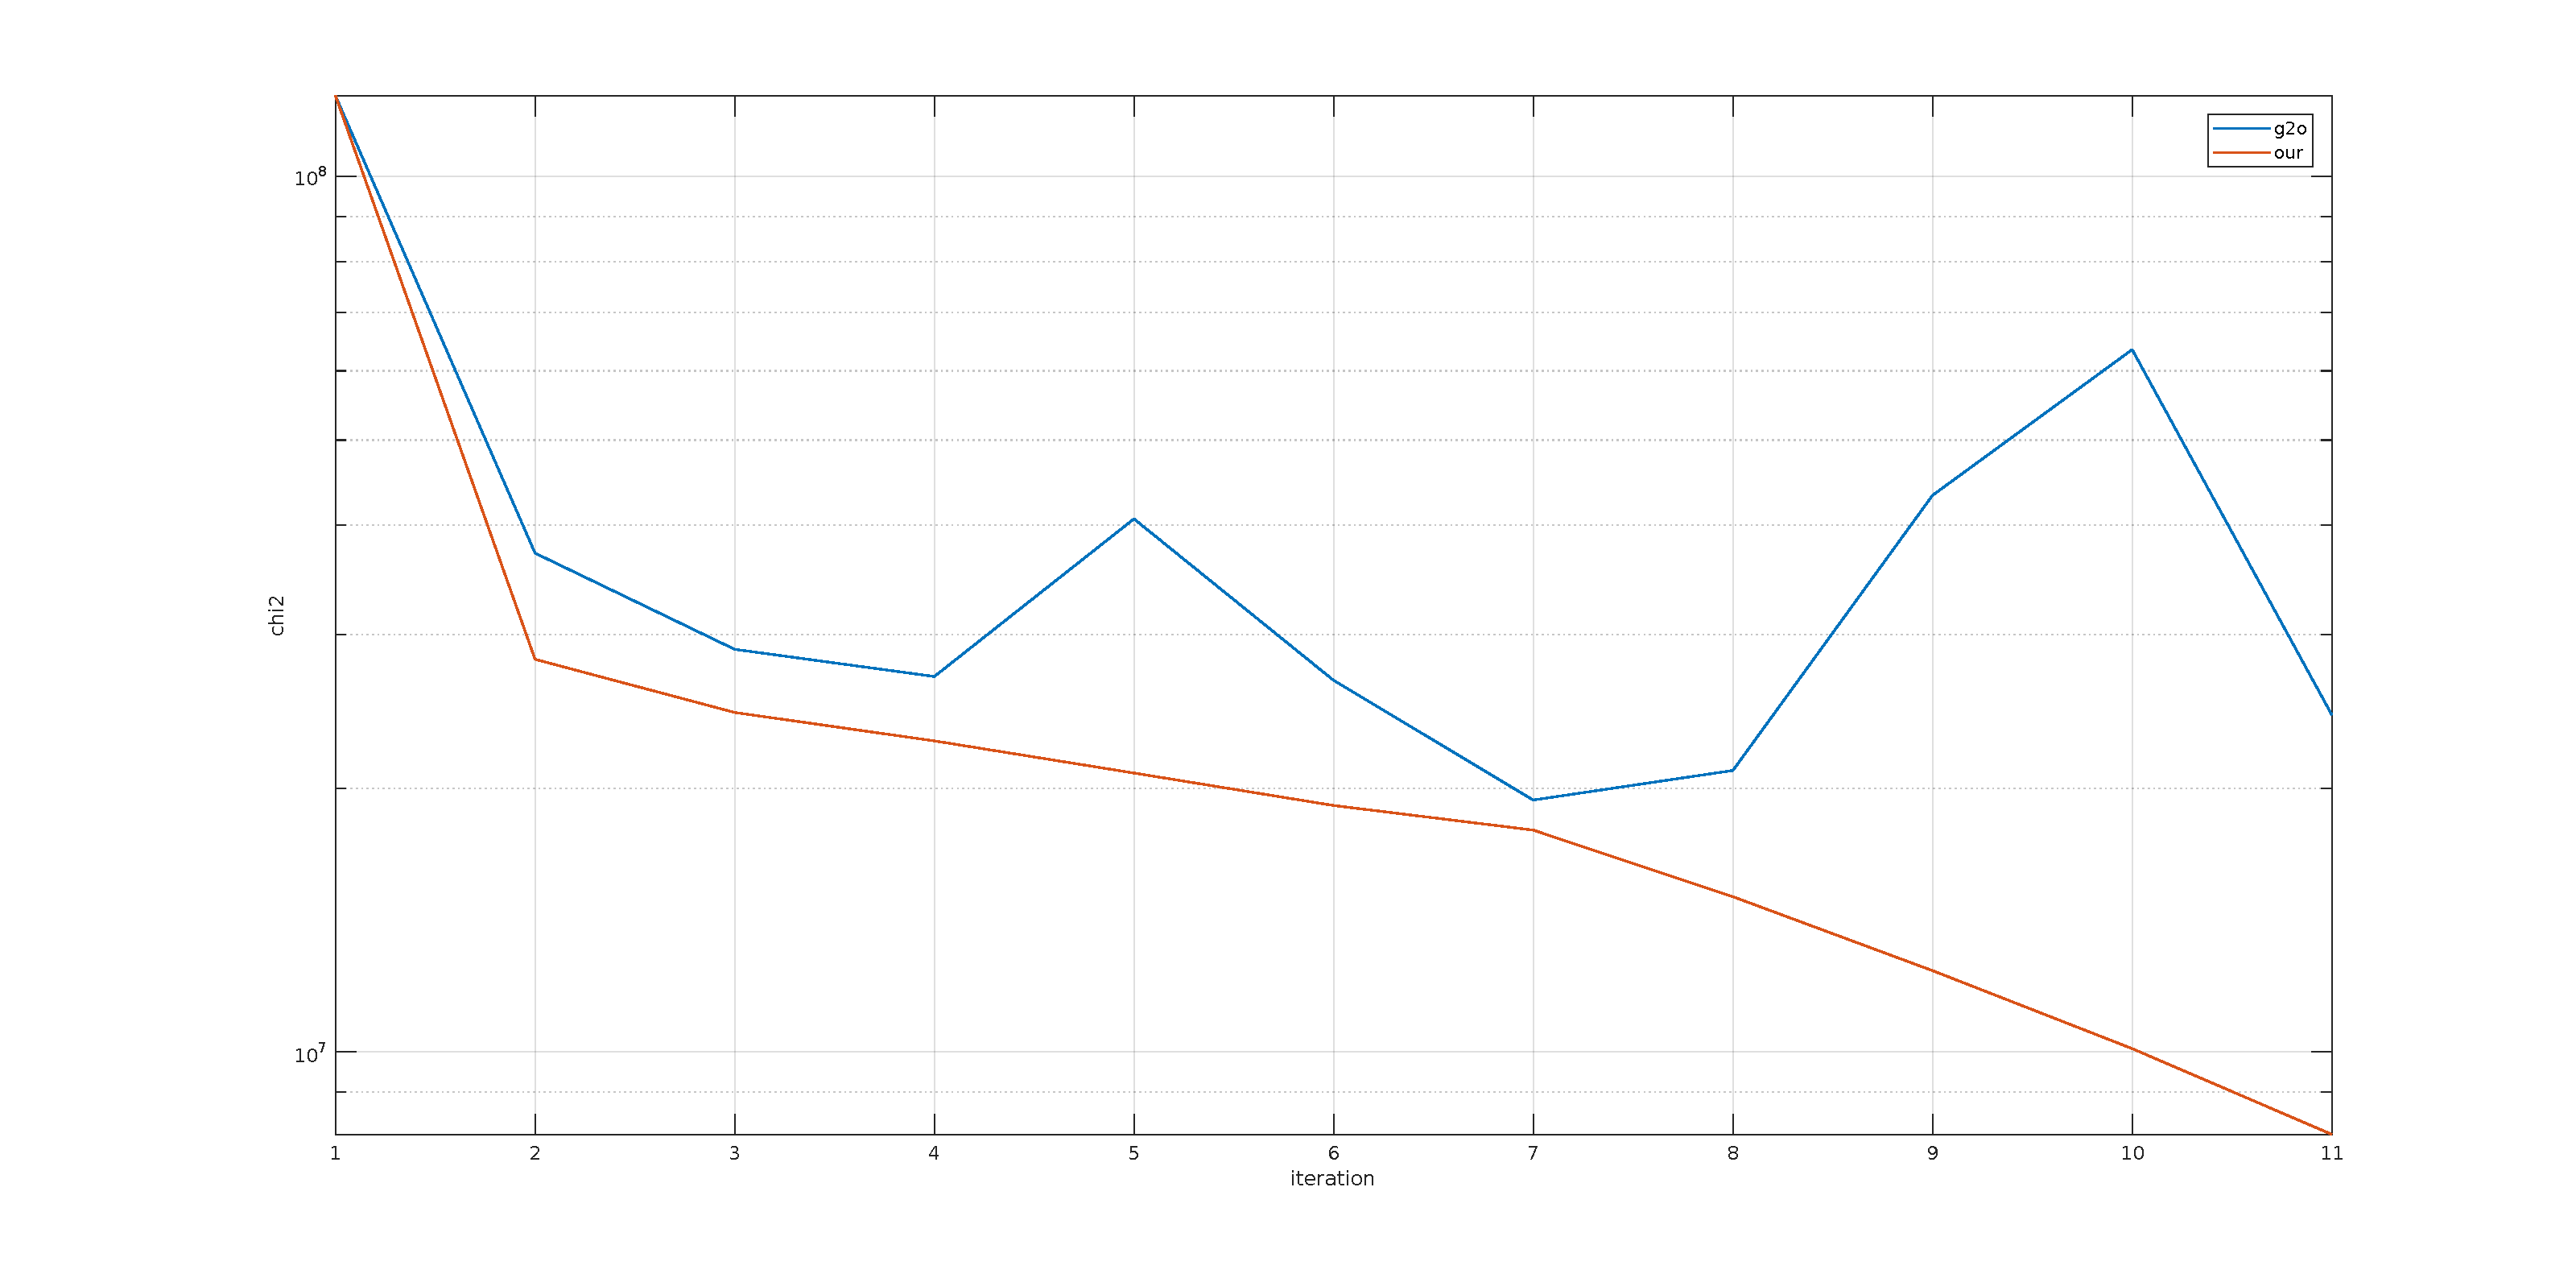
\includegraphics[width=\textwidth]{figures/04_solvingSe3/500p_N0_1e3R.pdf}
        \subcaption{}
        \label{fig:500p_gnadvanced_chi2}
    \end{minipage}%
    \caption{\textbf{Advanced Rotational Noise.} Figure (A) from left to right: \textit{initial guess}, \texttt{g2o} solution, \textit{our} solution. Figure (B) shows the \texttt{chi2} of both approaches at each iteration. \g2o's trend might indicate that the system got stuck in a local minimum.}
    \label{fig:500p_gnadvanced}
\end{figure}

The next step consists in applying both noise figures to the \textit{sphere} graph, together with a translational perturbation (therefore a 6 DoF noise vector), generating a very harsh initial guess.

\begin{figure}[!hbt]
    \centering    
    \begin{minipage}[t!]{0.9\textwidth}
        \centering
        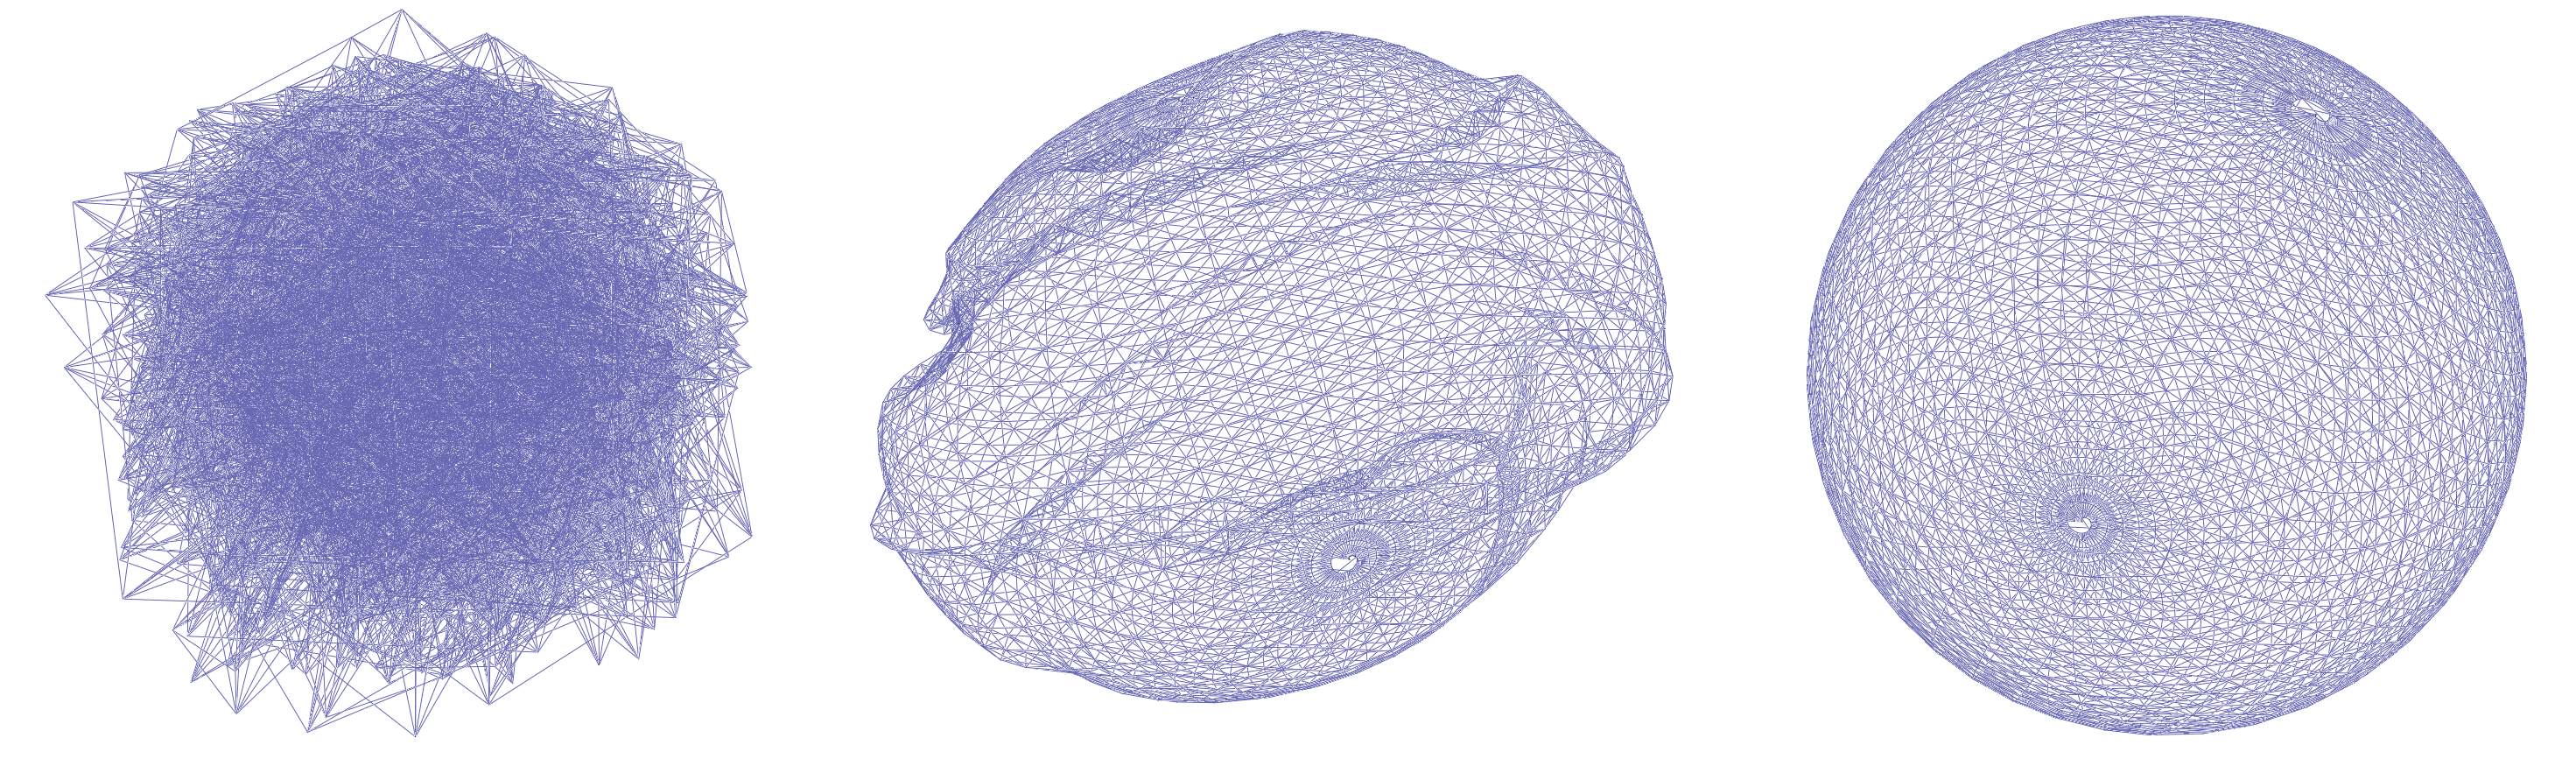
\includegraphics[width=\textwidth]{figures/04_solvingSe3/viewer_sphere_awgn_SOLVED.png}
        \subcaption{} 
        \label{fig:sphere_awgn_solution}
    \end{minipage}\\
    \begin{minipage}[t!]{0.9\textwidth}
        \centering
        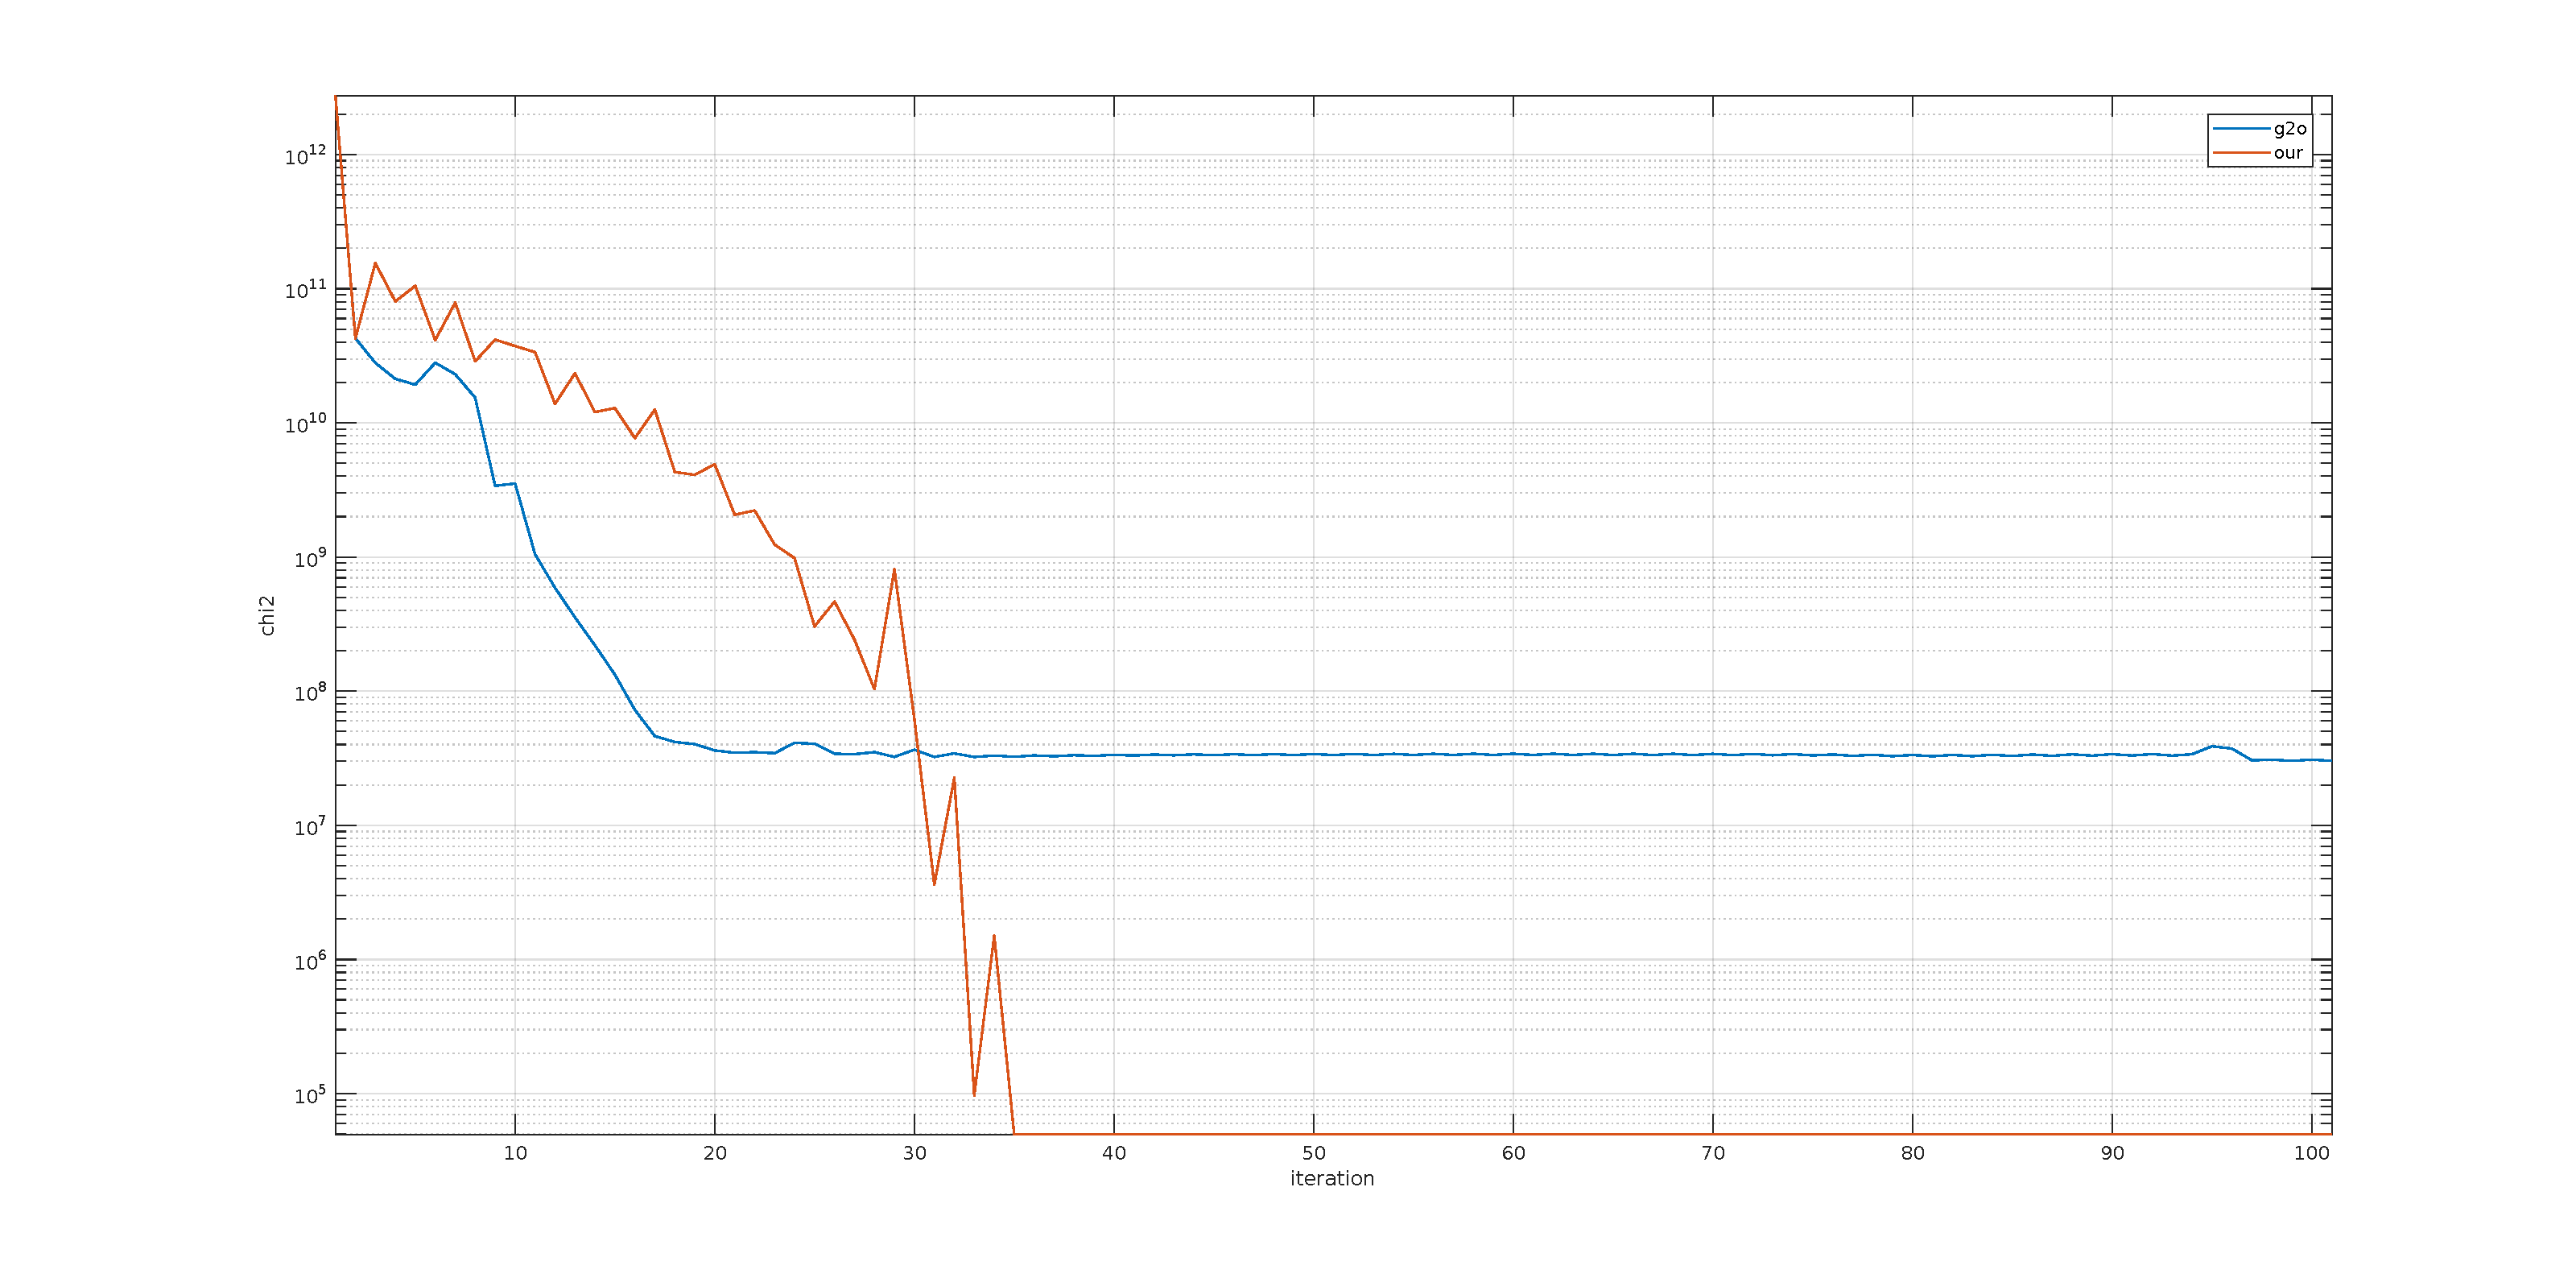
\includegraphics[width=\textwidth]{figures/04_solvingSe3/sphere_N0_1.pdf}
        \subcaption{}
        \label{fig:sphere_awgn_chi2}
    \end{minipage}%
    \caption{\textbf{Sphere 6 DoF Noise.} Figure (A) from left to right: \textit{initial guess}, \texttt{g2o} solution, \textit{our} solution. Figure (B) shows the \texttt{chi2} of both approaches at each iteration. From the plot it is clear that \g2o converges to a local minimum distant from the optimum. Here our approach instead is able to converge to the proper solution in less than 40 iterations.}
    \label{fig:sphere_awgn}
\end{figure}

\noindent Given the complexity of the initial guess, we decided to perform more iterations with respect the previous graph - i.e. 100. Figure \ref{fig:sphere_awgn} shows the qualitative and quantitative results of both \g2o and our approach, after applying 6 DoF Gaussian noise - sampled from $\mathcal{N}(0,1)$. The reader might appreciate the fact that \g2o converges to a \textit{local minimum} far from the optimum, instead, our approach is able to \textbf{reach the optimum in less than 40 iterations}.

Finally, in the last test it has been increased the rotational component of the noise, which, in this extreme case, is sampled from $\mathcal{N}(0,1)$. Here, without a kernel both the systems struggles to optimize the graph.

\begin{figure}[!hbt]
    \centering    
    \begin{minipage}[t!]{0.45\textwidth}
        \centering
        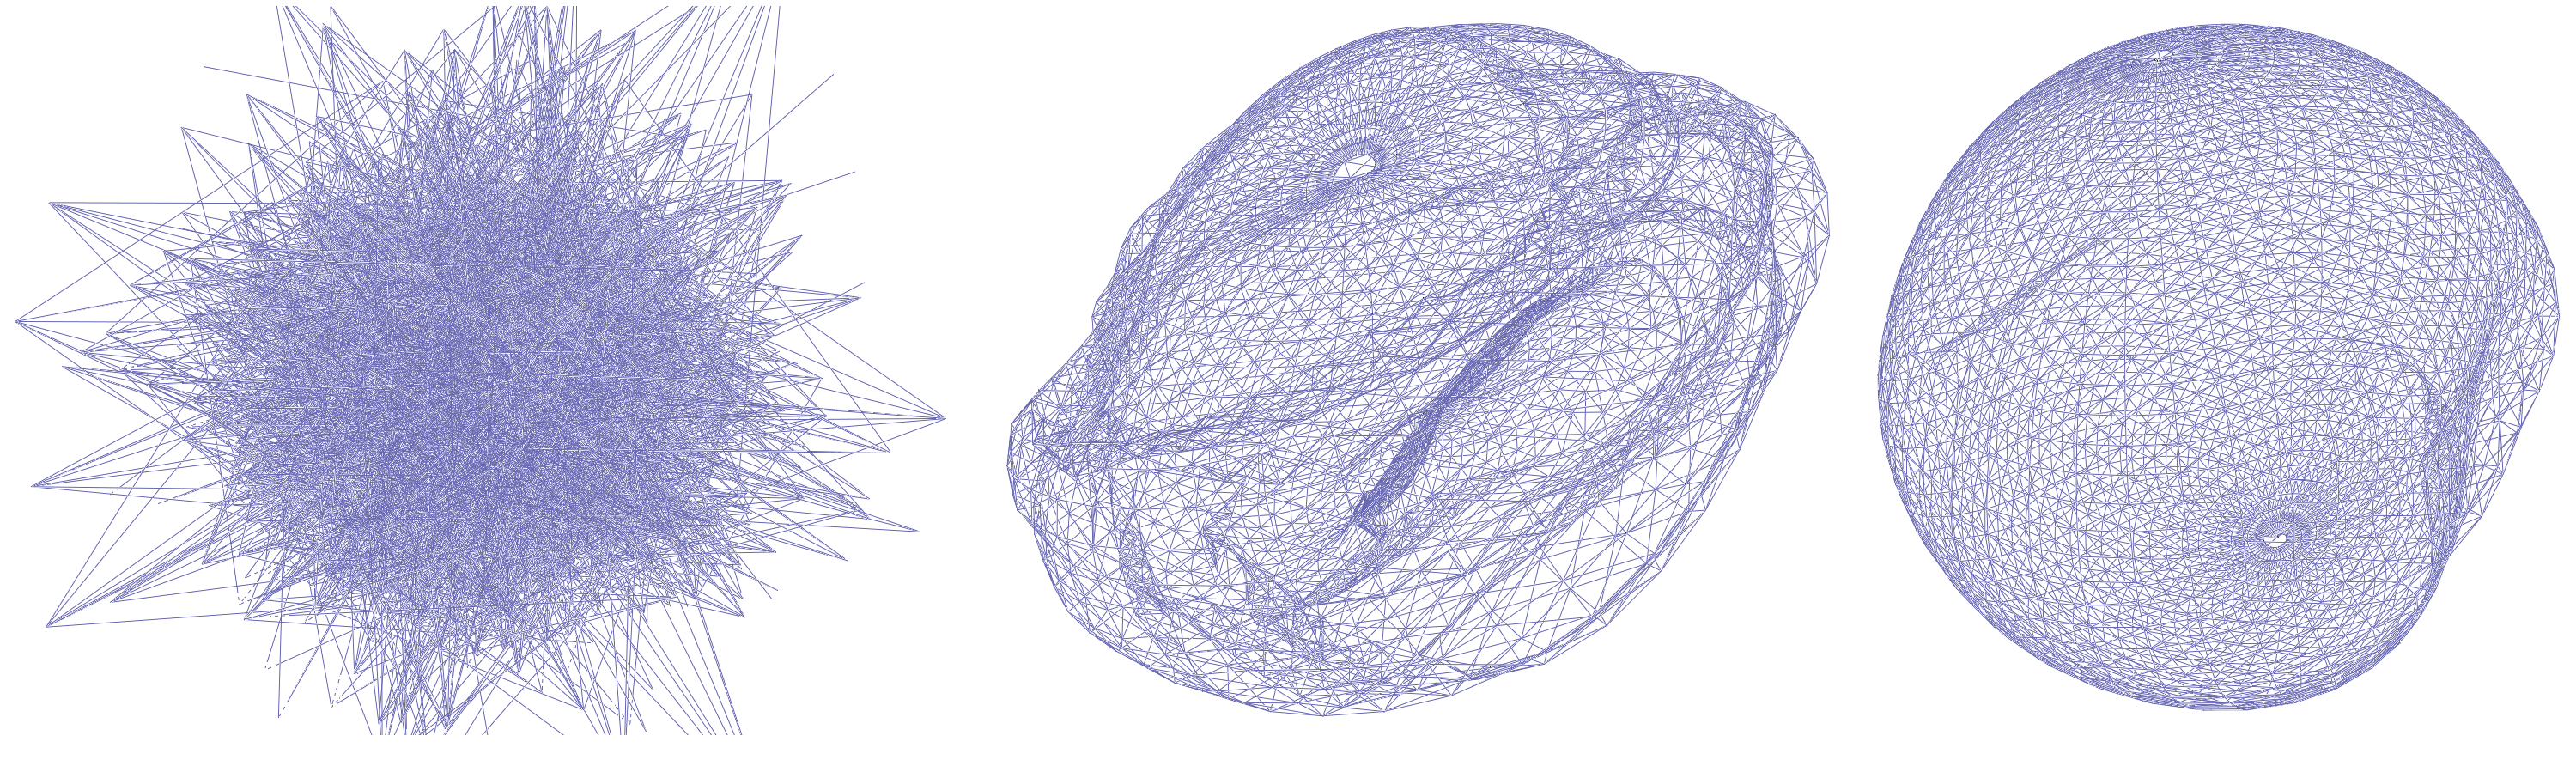
\includegraphics[width=\textwidth]{figures/04_solvingSe3/viewer_sphere_gnadvanced_SOLVED.png}
        \subcaption{} 
        \label{fig:sphere_gnadvanced_solution}
    \end{minipage}
    \begin{minipage}[t!]{0.45\textwidth}
        \centering
        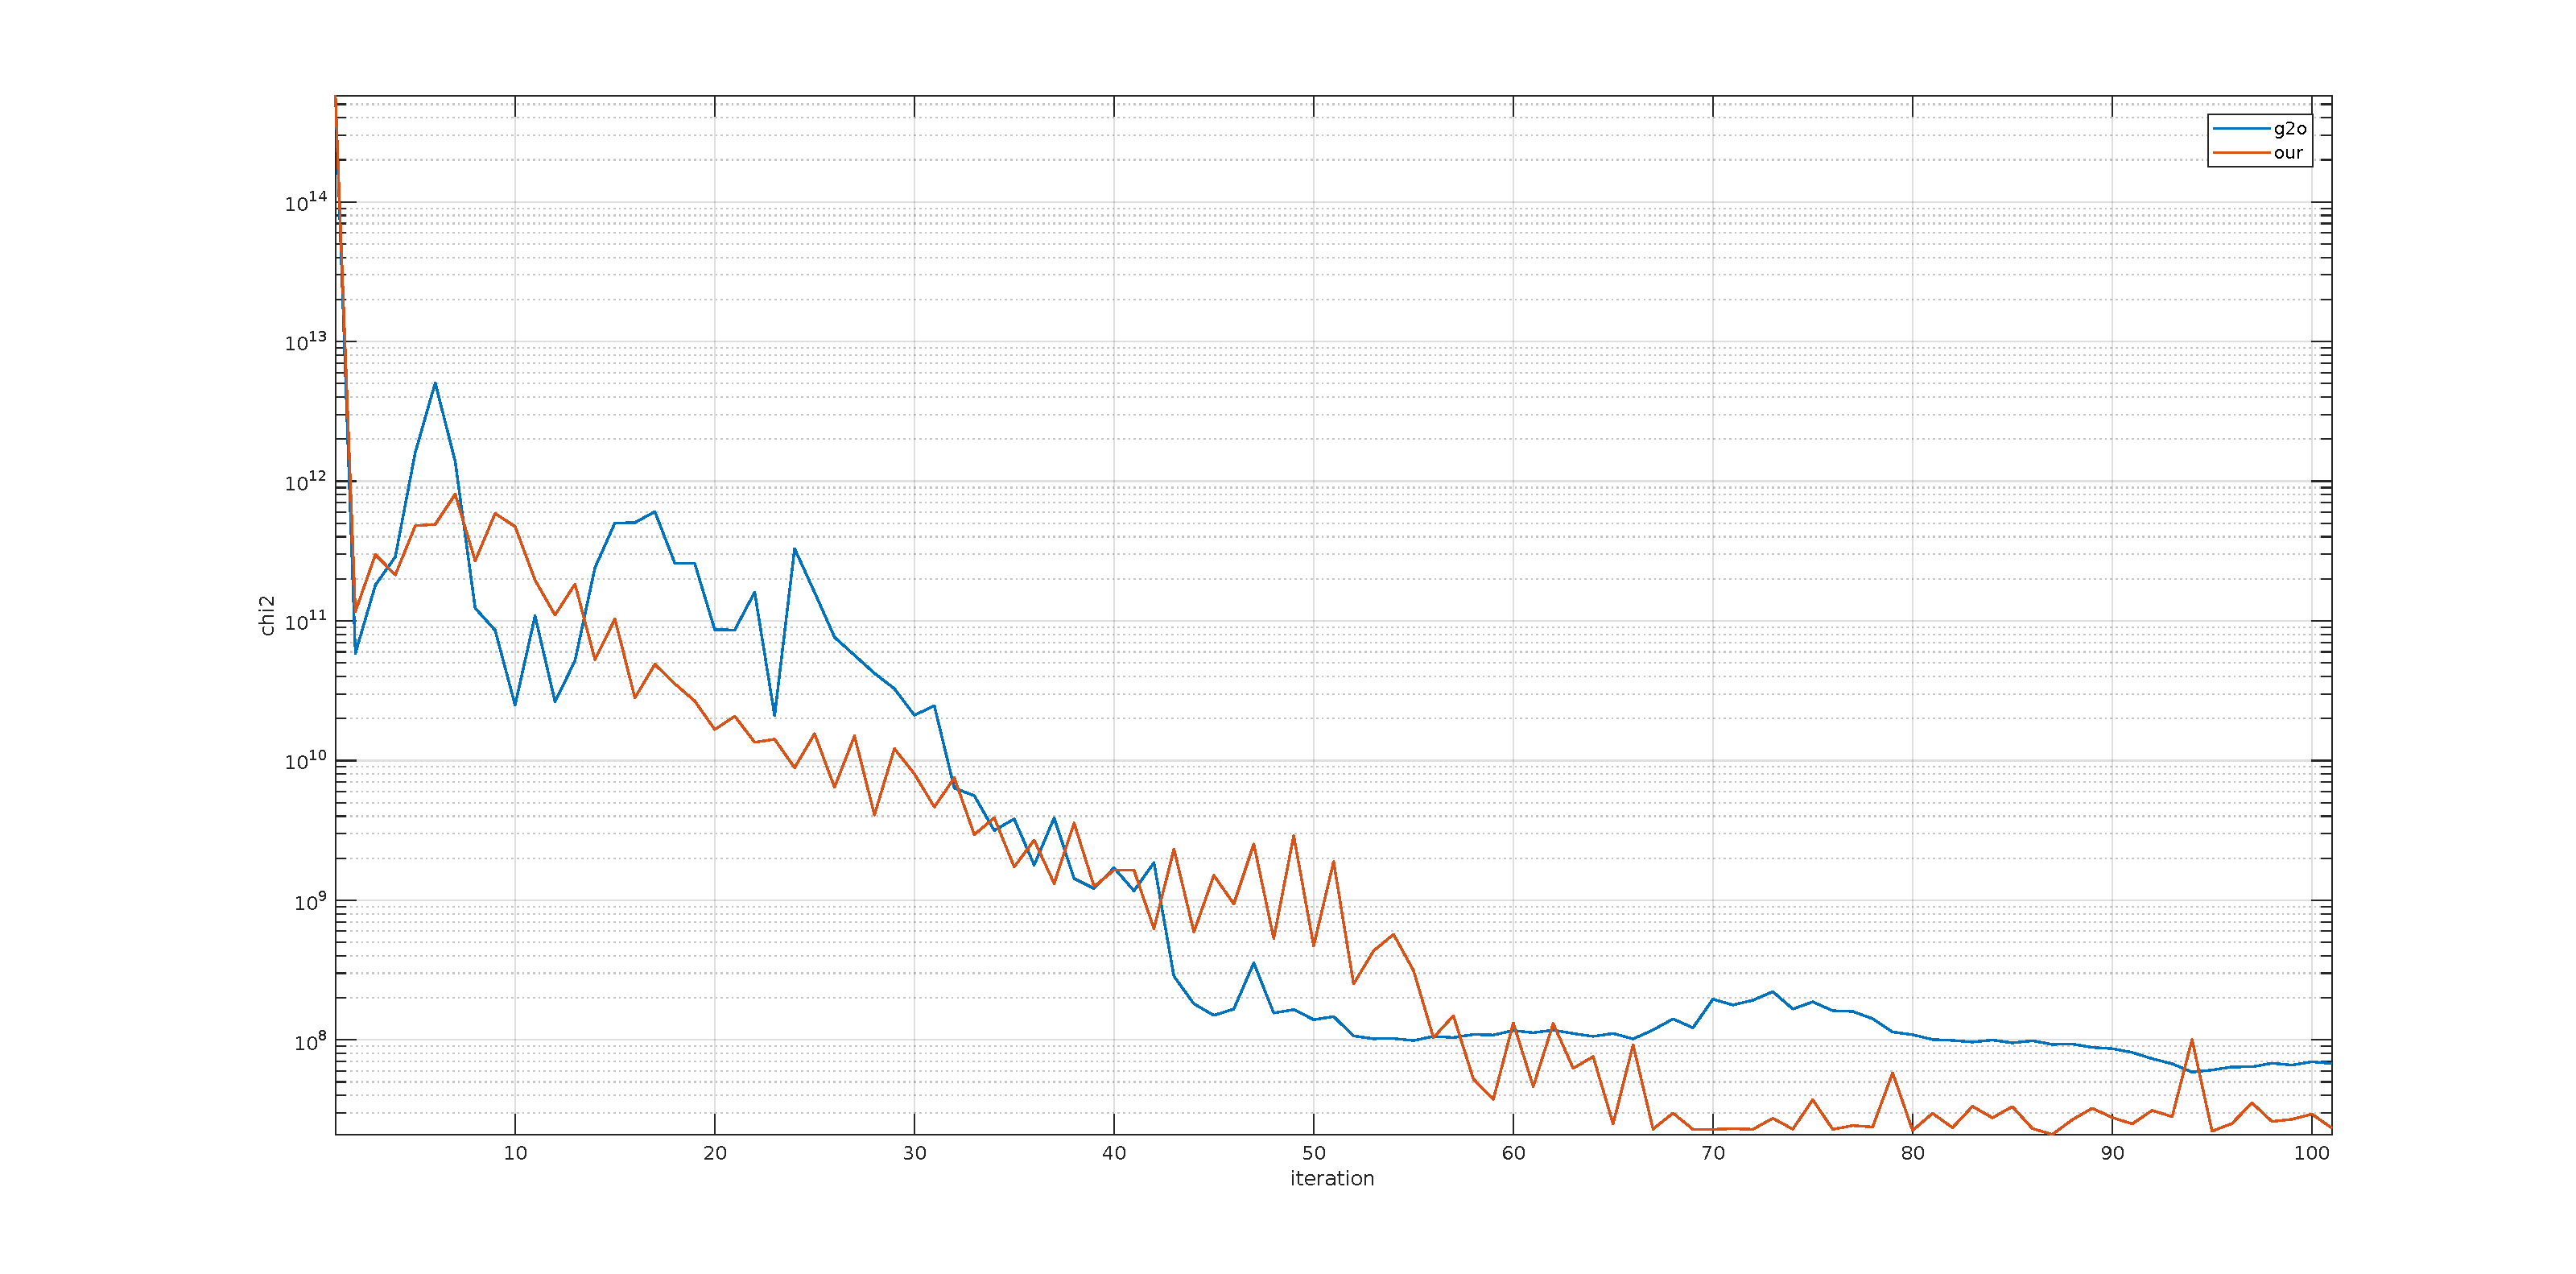
\includegraphics[width=\textwidth]{figures/04_solvingSe3/sphere_N0_1e3R.pdf}
        \subcaption{}
        \label{fig:sphere_gnadvanced_chi2}
    \end{minipage}%
    \caption{\textbf{Advanced Rotational Noise.} Figure (A) from left to right: \textit{initial guess}, \texttt{g2o} solution, \textit{our} solution. Figure (B) shows the \texttt{chi2} of both approaches at each iteration. Even if both systems fail in reaching the optimum, our system is able to generate a fair solution that can be further refined to reach the proper convergence.}
    \label{fig:sphere_gnadvanced}
\end{figure}

Figure \ref{fig:sphere_gnadvanced} shows the outcomes of both the systems: clearly neither \g2o nor our system reached the optimum, however the solution retrieved with the proposed method is evidently more consistent.

In Subsection \ref{subsec:benefits}, it has been highlighted that converting the information matrices from a 6-dimensional space to a 12-dimensional one through the \textit{Unscented Transform} may generate multiple rank loss, thus, the matrix $\bar{\Sigma}_k = \bar{\Omega}_k^{-1}$ must be conditioned somehow to avoid singularities. Given this, it has been tested the effects of different conditioning methods, however the most promising ones where basically 3:

\begin{enumerate}
    \item \textbf{Soft Conditioning.} It is computed the \textit{Singular Value Decomposition} of matrix $\bar{\Sigma}_k = UDV^\star$, then it is added a \textit{non-zero} value $\epsilon$ only to the degenerated eigenvalues and finally it is computed the matrix $\bar{\Sigma}_k^{conditioned} = U\tilde{D}V^\star$.
    \item \textbf{Mid Conditioning.} This is the method actually used to obtain the results seen until now, and consists in applying a non-zero value $\epsilon$ to all the elements on the diagonal of $\bar{\Sigma}_k$. Reasonable values are $\epsilon \in [10^{-2}, 10^{-4}]$.
    \item \textbf{Hard Conditioning.} In this case, all the values outside the main diagonal are simply ignored - i.e. set to zero. 
\end{enumerate}

\begin{figure}[!hbt]
    \centering    
    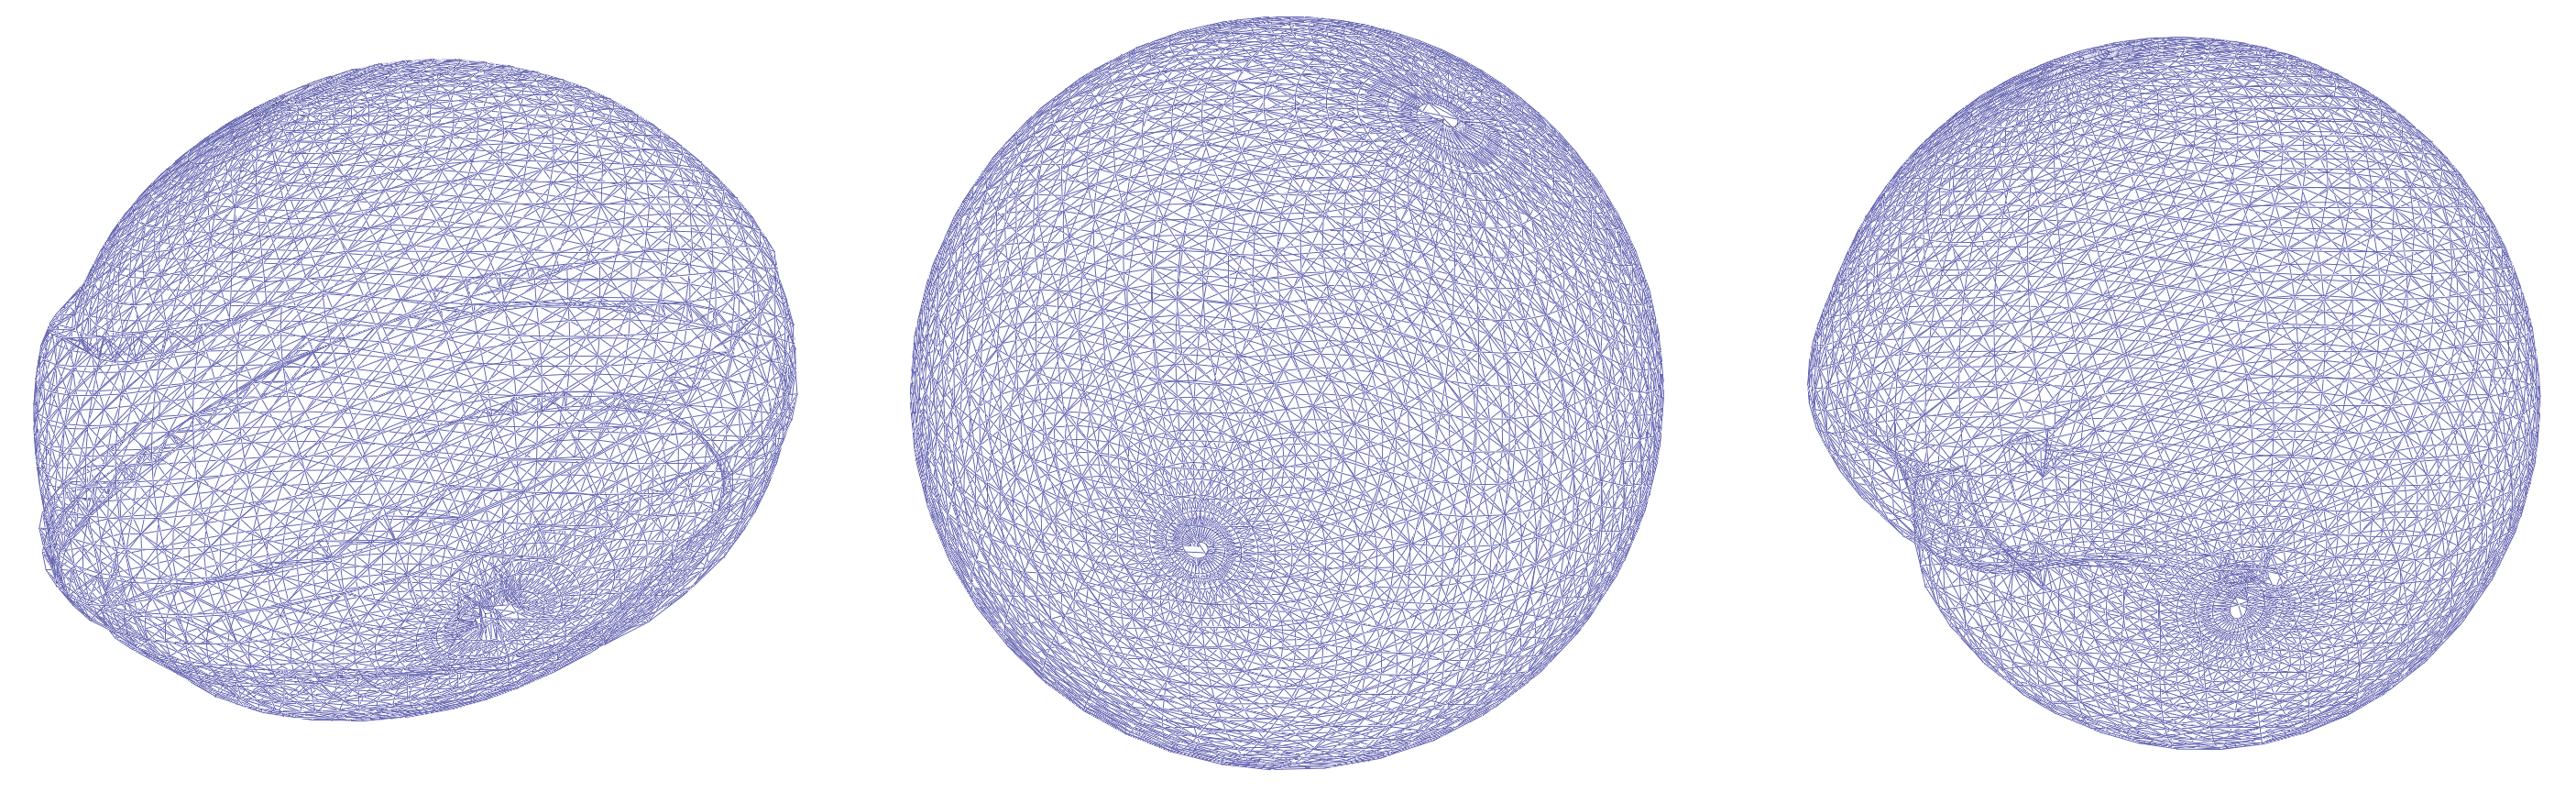
\includegraphics[width=0.7\textwidth]{figures/04_solvingSe3/viewer_sphere_awgn_CONDITIONINGS.png}
    \caption{\textbf{Conditioning Methods.} The outcomes of the three conditioning methods used to compute the measurements' information matrix. Given the initial guess relative to Figure \ref{fig:sphere_awgn_solution}, from left to right are illustrated: soft, mid and hard conditioning.}
    \label{fig:sphere_conditionings}
\end{figure}

This comparison opens a new path for further investigations, in order to retrieve the best conditioning method to compute the measurements' information matrices.

\vspace{15px}

As this Section showed, the novel features introduced so far lead to an accurate and more robust optimizer, that delivers results \textbf{comparable or better} to other state-of-the-art systems. In the next Chapter, the reader will have an insight on the actual implementation of the system, in order to better understand how all those mathematical concepts have been applied in practice and to show the speed performances reached by our system.